\documentclass[12pt]{article} 
\usepackage{a4}
\usepackage{isolatin1} 
\usepackage{amsmath} 
\usepackage{bbm}
\usepackage{epsfig} 
\newcounter{figcount}
\begin{document}
\section{The MathletFactory from a System Developer's Perspective}
\label{implementation_details}
This appendix contains an overview of the MathletFactory from a system developer's perspective. This perspective
is necessary for developing new MMObjects or display components that extend the set of mathematical entities represented by 
the MathletFactory.\\
In the following sections we omit the details, which can be found at the API documentation but give a structural overview that 
follows the Model-View-Controller architecture.
\subsection{MVC Architecture of the MathletFactory}
\subsubsection{Requirements}
Following the didactic model of Bruner, mathematics can be regarded as a system with three complementing representations: 
The {\it enactive} representation of a mathematical entity is determined by what you can {\it do} with it, the 
{\it iconic} representation is an image or sketch that {\it visualises} one or more of its properties and the 
{\it symbolic} representation {\it denotes} it in a formal language system. One of the main conclusions of Bruner's Theory 
is, that although professional mathematicians almost exclusively use symbolic representations, the other types of representations 
play a vital role in learning mathematics.\\
If we use this didactic principle as a requirement for the architecture of a mathematics learning framework, it makes 
sense to allow different representations for mathematical objects. This can be done best by using the 
Model-View-Controller Pattern\footnote{\cite{Bu96}}, an architectural pattern that separates the data of an entity from 
its presentation and application logic.

\subsubsection{Fundamental Concepts}
A good starting point when describing the MathletFactory is to describe what happens, when a student uses an applet
created with the MathletFactory.\\
If, for example, a student drags the graphical representation of a three dimensional vector on a canvas with the
mouse, the canvas generates an event that is sent to the {\tt CanvasController}. This instance checks all objects
contained in the canvas if they are meant, by using the mouse coordinates and the canvas' internal projection 
parameters. If an object has been picked and it can handle the type of event (by owning an appropriate handler), the 
event is delivered to it by calling {\tt MMObjectIF.doAction()}. The {\tt MMObject} then delegates the event to the 
specified handler, which processes the event (e.g.\ translating the end-point of the vector in a plane parallel to 
the viewport by transforming the new mouse coordinates to world coordinates) and modifies the state of the 
{\tt MMObject} (e.g.\ setting its coordinates to new values). After this it is checked, if any other objects depend 
on the vector (for example, the vector could be designated as normal for a plane). For this it is checked, if any 
{\tt Updater}s are associated to the object and if so, their {\tt update()} method is called, changing the state 
of any dependent objects (which in turn might also have other updaters and so on). After the update graph traversal 
has been finished, The views of the objects that were changed, are redrawn (both the graphical and the symbolic 
representation), by invoking {\tt render()} and {\tt draw()} in all transformers of the {\tt MMObject}. By this
the student is informed of the result of his action and may proceed with further actions.

\stepcounter{figcount}
\begin{center}
\resizebox*{16cm}{!}{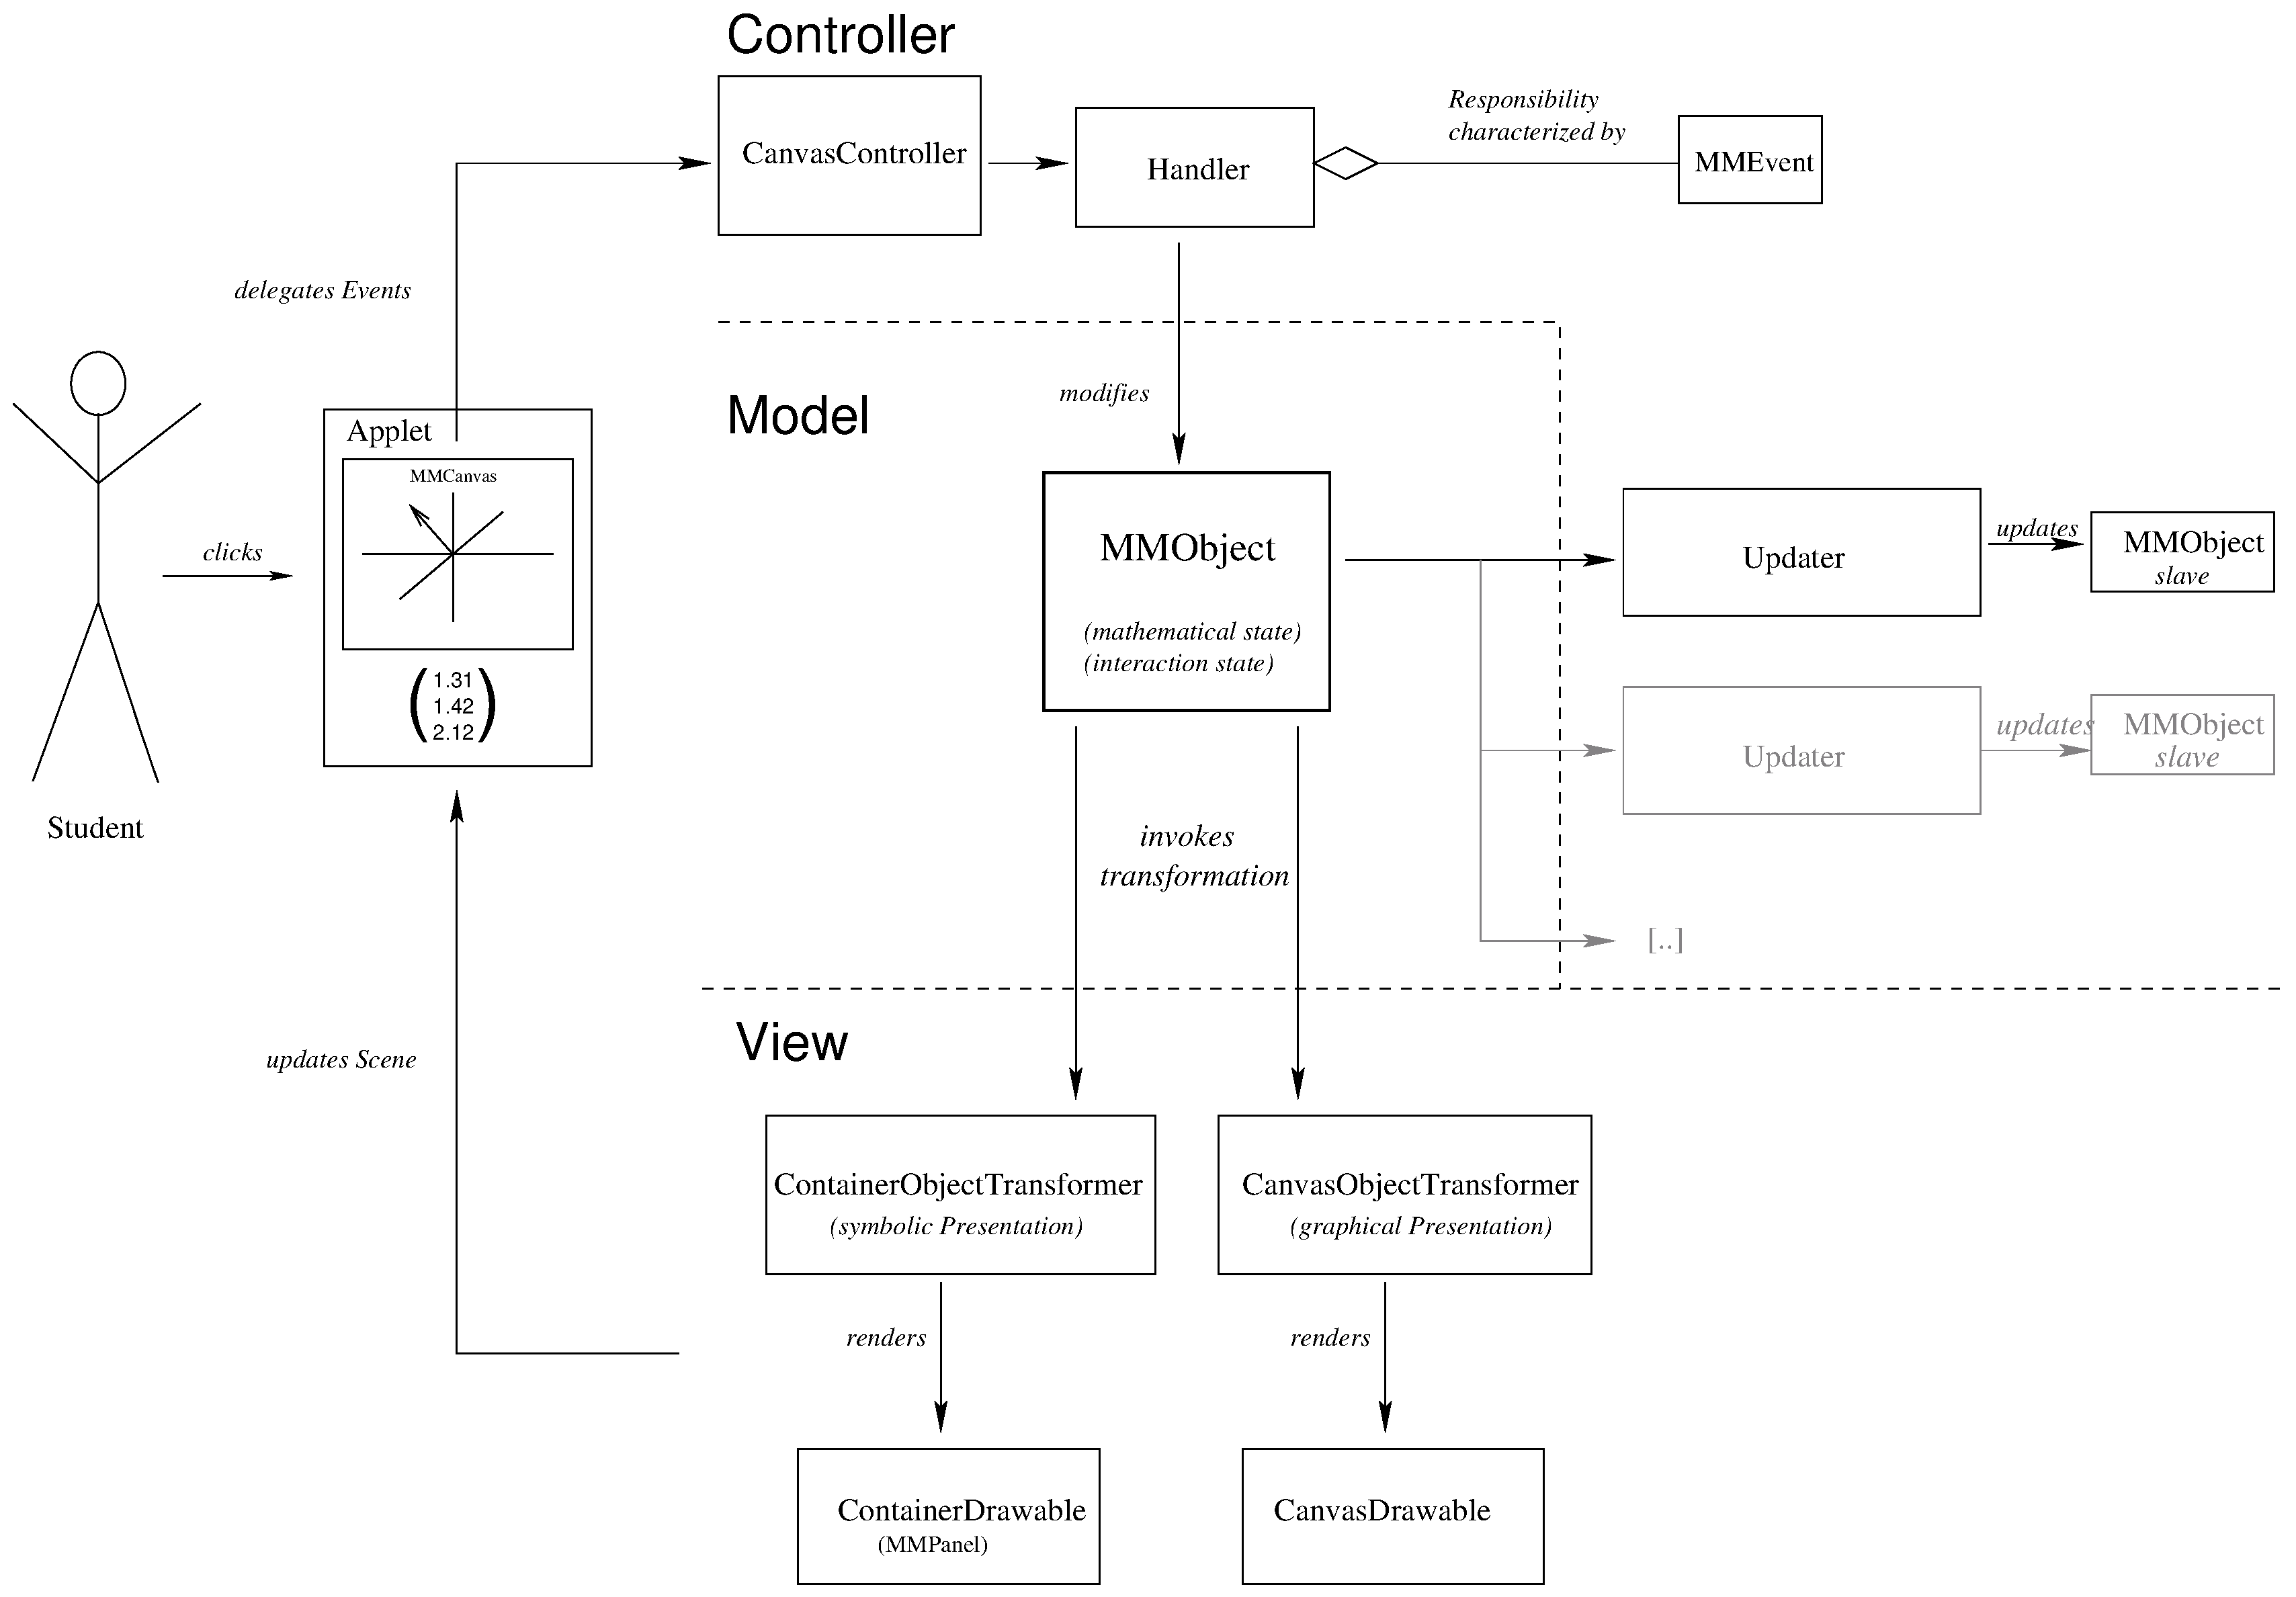
\includegraphics{mvc}}\nopagebreak\\[1.0cm]\nopagebreak
\footnotesize{{\sf Fig.\ \arabic{figcount}: An action cycle in the MVC architecture }}\\[0.6cm]
\end{center}

\subsubsection{Model}
The core model used in the MathletFactory is the {\it MMObject}, represented
by a class that implements the {\tt MMObjectIF} interface. An instance of this class contains on the one hand the mathematical 
information of the object, on the other hand it also owns references to the handlers that allow its manipulation and to updaters
that connects the object with other MMObjects in the update graph. It also contains the link to the view components.

\subsubsection{View}
The view component consists basically of two objects: The {\it transformer} (represented by a subclass of {\tt GeneralTransformer})
the {\it drawable} (represented by the interface {\tt Drawable}). While the drawable is the actual displaying unit, the 
transformer establishes a link between model and drawable and knows how to repaint it, when the MMObject has changed.

\subsubsection{Controller}
In the controller section we differentiate between objects that directly manipulate MMObjects and those that are responsible
for constructing the update graph. The directly manipulating objects are represented by two different classes: Handlers (subclasses 
of {\tt MMHandler}) for manipulating iconic representations in a canvas (e.g.\ selecting and dragging vectors with the mouse) and 
panels (subclasses of {\tt MMPanel}) for editing symbolic representations. Note that the panel is also a drawable into which
the controller-code (which consists of only a few lines) has been integrated into.\\

\subsection{Arithmetic and Geometric Model}
In order to compute a wide variety of mathematical problems, the Mumie MathletFactory offers a flexible and economic model for
representing the geometric and arithmetic properties of mathematical entities and allows an accessible interface for easy 
manipulation. In the following, we briefly describe the model architecture of the basic entities. 

\subsubsection{Number Types}
Starting with the specification that all mathematical objects -- directly or indirectly -- use numbers, we assign to each MMObject a
specific number type that can be changed upon construction or sometimes even at run time. By this it is, for example, possible 
to use the same sequence object for displaying both real valued sequences and complex valued sequences. In the first case
the object is instantiated by invoking the constructor with the argument {\tt MComplex.class}, the second with the argument 
{\tt MDouble.class}. The implementation is done using an abstract base class {\tt MNumber} of which all number types
are subclasses. Currently, the following number types exist:\\

\stepcounter{figcount}
\begin{center}
\begin{tabular}{|p{5cm}|p{3cm}|p{5cm}|}
\hline
Number Type & Set of numbers modelled & Internal Java type used\\
\hline
{\tt MNatural} & $\mathbbm{N}$ & {\tt BigInteger}\\
\hline
{\tt MInteger} &  $\mathbbm{Z}$ & {\tt double}\\
\hline
{\tt MRational} &  $\mathbbm{Q}$ & {\tt long}\\
\hline
{\tt MBigRational} &  $\mathbbm{Q}$ & {\tt BigInteger}\\
\hline
{\tt MDouble} &  $\mathbbm{R}$ & {\tt double}\\
\hline
{\tt MComplex} &  $\mathbbm{C}$ & {\tt double}\\
\hline
{\tt MZmod5} & $\mathbbm{Z}/5\mathbbm{Z}$ & {\tt int}\\
\hline
\end{tabular}
\end{center}

The last is an experimental type that demonstrates the use of finite fields in the MathletFactory and will soon be replaced
by a generic class modelling $\mathbbm{Z}/p\mathbbm{Z}$.

\subsubsection{Vectors, Vector spaces and Matrices}
While the subclasses of {\tt MNumber} provide the base for one-dimensional number computing, the class {\tt NumberMatrix} --
representing an $m\times n$-matrix -- is fundamental for the calculation in linear spaces of higher dimension. As MMObjects 
it has also exclusively uses the generic number interface allowing each instance of a {\tt NumberMatrix} to represent a 
matrix of different number type.\\
The {\tt NumberMatrix} is extended by {\tt NumberTuple}, a class that represents  $m\times 1$-matrices and which is basically 
used as coordinates for vectors or matrix columns/rows. It therefore offers additional functionality like the norm, the dot 
product, etc.\\
Vectors in turn are modelled by subclasses of the abstract {\tt NumberVector}. It is a specific trait, that each vector
of the MathletFactory `knows' the vector space in which it exists and is represented by coordinates that are relative to its
associated basis. By this it is possible to transform all vectors of a chosen vector space by changing the space's basis.
The {\tt NumberVectorSpace} class therefore provides a wide range of methods to manipulate its basis. 

\subsubsection{Affine and Projective Geometry}
The vector space model is also used in the geometric classes. Like most CAG (Computer Aided Geometry) Modelling software.
All internal data is stored in homogeneous (i.e.\ projective geometry) coordinates. This allows the easy transformation
of mathematical entities also for affine geometry. For example, when calculating the intersection of two planes in the
three dimensional space $\mathbbm{R^3}$ (i.e.\ the intersection of 2D affine subspaces within a 3D affine space) simply
the projective hyperplanes have to be intersected, reducing the problem to finding the null space of the matrix that 
contains the projective coordinates of the subspaces' basis (see extended description of this example below).

\subsubsection{Numerical Computing}
Numerically, almost all affine and projective geometric operations -- like the example above -- base on the Gauss algorithm 
implemented in the class {\tt EchelonForm}. This ensures a high reusage and offers an easy optimisation opportunity: If the 
Gauss algorithm is made faster, a wide range of computations will be executed faster.

\subsubsection{Compound Example}
To demonstrate, how all the concepts described above work together, we give a `real life' example: In the mathlet depicted
below, the intersection of two planes in three dimensional is computed and displayed (For details refer to the documented 
source code):

\begin{center}
\resizebox*{8cm}{!}{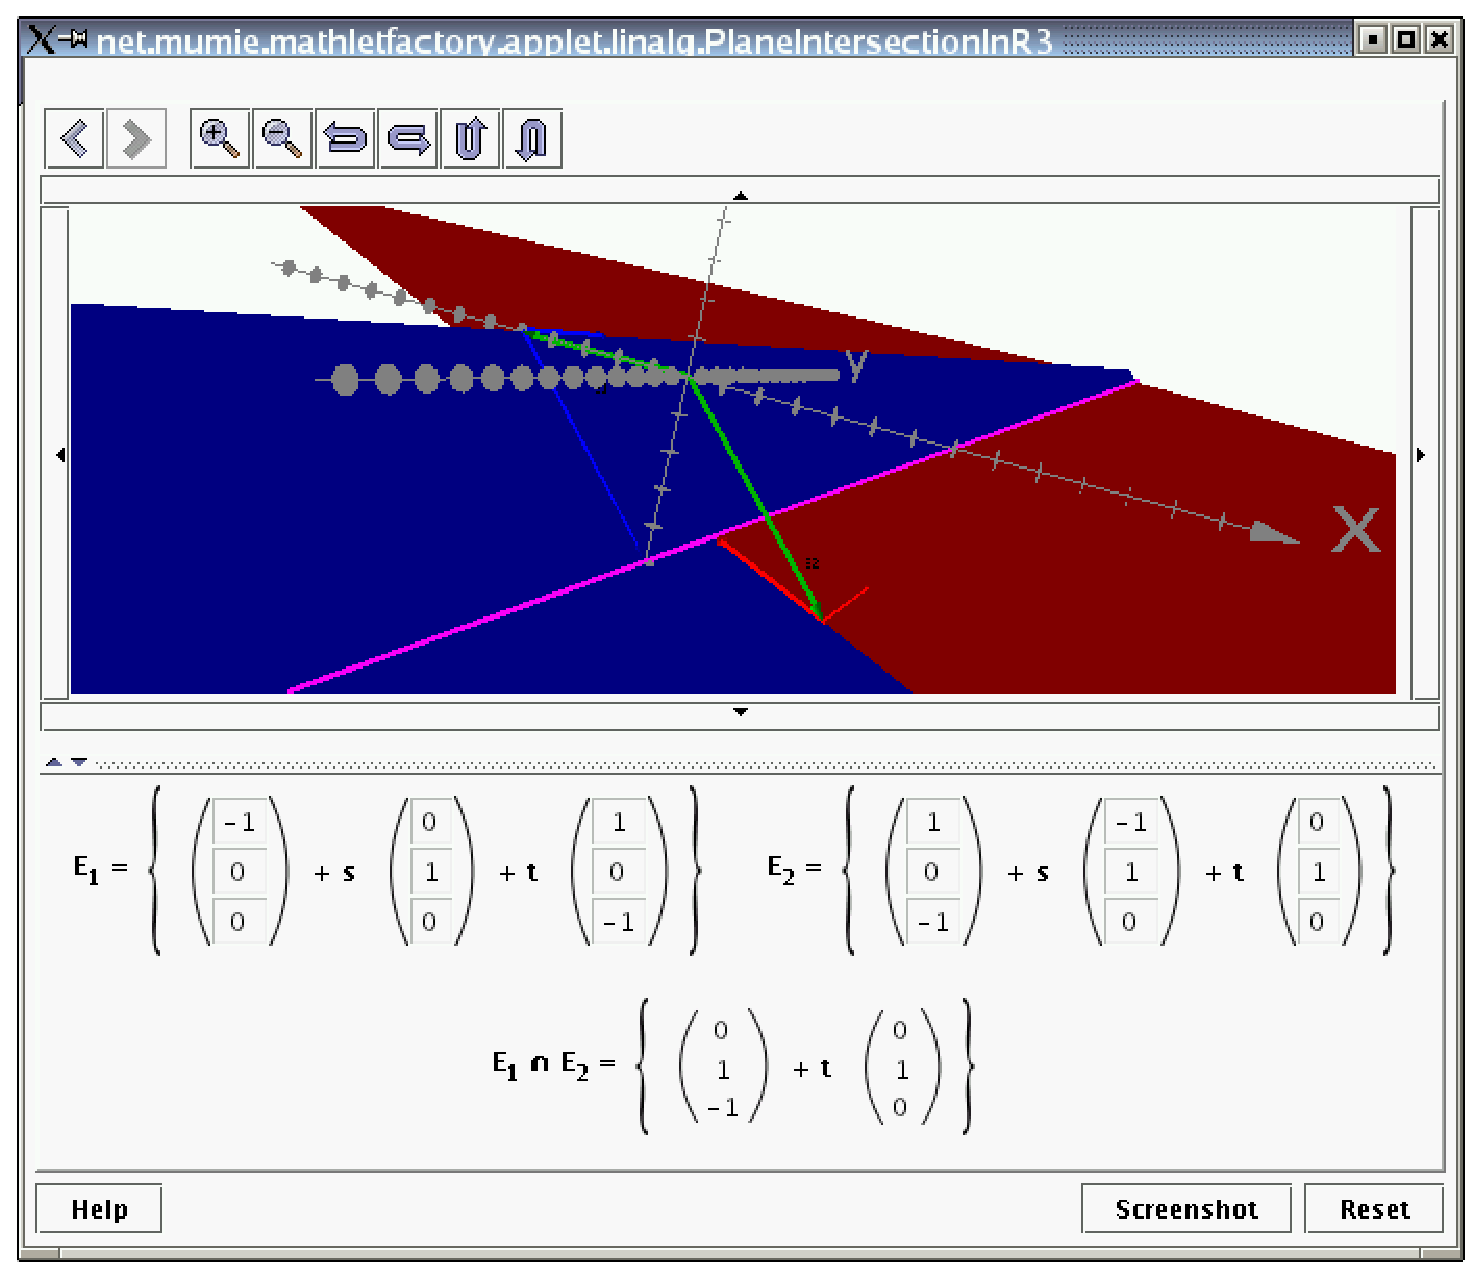
\includegraphics{PlaneIntersectionInR3}} \hspace{0.5cm} \begin{minipage}[b]{8cm}
\begin{footnotesize}
\begin{verbatim}
	AffineSpace.intersected()
                 |
	AffineSpace.intersect()
                 |
	ProjectiveSpace.intersected()
                 |
	NumberVectorSpace.intersected()
                 |
	SolveHomogen.intersection()
                 |
	SolveHomogen.nullSpace()
                 |
	EchelonForm.getREFMatrix()
                 |
	EchelonForm.toReducedRowEchelonForm()

\end{verbatim}
\end{footnotesize}
\end{minipage}\nopagebreak\\[0.5cm]\nopagebreak
\footnotesize{\sf Fig.\ \arabic{figcount}: The intersection of two planes in three-dimensional space and its stack trace to the Gauss algorithm}\\[0.3cm]
\end{center}

This starts in by invoking the method {\tt AffineSpace.intersected(AffineSpace with)} in one of the planes
with the other as argument (the plane class descends from the affine space class). This method does nothing but the
invocation of its projective representation to intersect with the projective representation of the other plane.
This is done by giving their two vector bases to the method {\tt SolveHomogen.intersection(NumberTuple[] span1, NumberTuple[] span2)}
which in turn calls the {\tt nullSpace(NumberMatrix matrix)} method with a (3$\times$6) matrix as argument that contains all the 
base vectors as columns. This method in turn uses the Gauss algorithm implemented in {\tt EchelonForm.getREFMatrix(NumberMatrix matrix)}
to transform the matrix to reduced echelon form to determine its null space basis. The null space basis is then used as parameters 
for constructing the basis of the intersecting space, which is returned by the {\tt intersected()} method.

\section{Algebraic Object Model and Formal Languages}
Since often it is not only needed to let the application developer perform computations with the MathletFactory but also the 
student (or teacher/tutor) himself, the arithmetic and geometric model is complemented by an algebraic model that allows the 
input of expressions in a formal language. By this, the flexibility of the mathlets is increased and allows them to be used
as tools in open learning scenarios.

\subsubsection{Lexical, Syntactic and Semantic Analysis}
In order to analyse and interpret a formal language, we need structures that operate on three different levels of language: the first 
is the lexical analysis which analyses the alphabet of symbols being used, the second is the syntactic analysis that applies
the rules for building words and sentences. On the third level we have the semantic analysis that analyses the meaning of the
words.\\

\stepcounter{figcount}
\begin{center}
\resizebox*{15cm}{!}{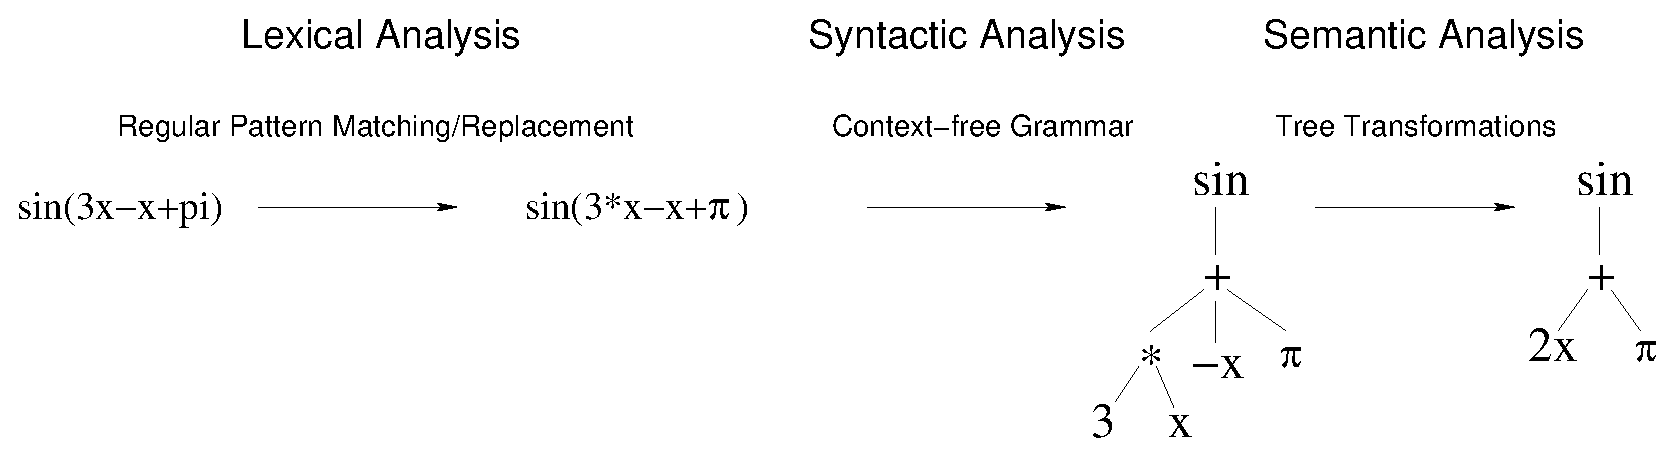
\includegraphics{languageProcessing}}\nopagebreak\\[0.5cm]\nopagebreak
\footnotesize{\sf Fig.\ \arabic{figcount}: The different stages in mathematical
  expressions analysis performed by the MathletFactory}\\[0.6cm]
\end{center}

In the MathletFactory, each stage of language processing is performed by a specific unit: The lexical analysis is performed by 
a set of regular expressions (which also do some replacements that allow an increased robustness like {\tt 2x} $\rightarrow$ 
{\tt 2*x}) and a small scanner unit. The syntactic analysis is done by a parser that implements a context-free grammar (see below) 
and the semantic analysis is left to a rule-based tree automaton that operates on the operation tree generated by the parser.\\
Note that it is quite easy to reproduce a string out of the tree representation by doing a depth-first 
order traversal, thus closing the sequence to a loop. This is very important for interactive work with mathematics, where the user 
enters an expression, watches the response of the system and may want to re-edit his input for a receiving a different result.
\subsubsection{Introduction to Formal Languages}
The main idea of the MathletFactory's algebraic object model takes advantage of the formal languages used in mathematics. 
Computer science has developed a rich set of methods to interpret these formal languages of which we can only give a 
short introduction, see \cite{HU79} for details.\\
A formal language can be defined as a concatenation of symbols from an alphabet. These concatenations are called the 
{\it words}. The formal language ${\cal L}(\Sigma)$ over an alphabet $\Sigma$ that consists of all possible words can thus inductively
be defined as:

\begin{enumerate}
\item $\sigma \in {\cal L}$ for all $\sigma \in \Sigma$.
\item $w \in {\cal L}$ for $w = u.\sigma$ with $u \in {\cal L}, \sigma \in \Sigma$.
\end{enumerate}

with $.$ being the concatenation operator. The language that consists of all words over $\Sigma$ is also called 
$\Sigma^*$, where the $^*$-operator means, that the resulting set contains all finite concatenations 
$\sigma_1.\sigma_2\ldots\sigma_n, n \in \mathbbm{N}$ of symbols $\sigma_i \in \Sigma$, and the empty 
word $\varepsilon$.\\

Of course we are more interested in languages that allow only certain words. For example, we may want {\tt (x+1)} to be a 
word of our language, but not {\tt +)1)x}. We thus need a higher structure that tells us, which words belong to the language, a 
{\it grammar}.\\ 
A grammar is defined by the accepted alphabet (the {\it terminals}) and by a set of explicit rules how a word can be decomposed 
into these. For example, one could state the following rules for simple arithmetic expressions of numbers represented by
{\tt NUM}:\\ 
\renewcommand{\thefootnote}{\fnsymbol{footnote}}

\begin{enumerate}
\item {\tt +}, {\tt -}, {\tt *}, {\tt /} $\in {\cal L}$,  {\tt NUM} $\subset {\cal L}$,\footnote{Note, that for avoiding trivial rules 
it is better to regard a number like {\tt 1234} to be represented by a single symbol, not as a concatenation of symbols as one would 
presume by the fact that it is a concatenation of digits in our common writing system. In the following we will also regard function 
identifier like {\tt cos} as a single symbol in order to keep our grammar compact.}
\item $w \in {\cal L}$ for $w = u.${\tt *}$.v$ or $w = u.${\tt /}$.v$ with $u,v \in {\cal L}$,
\item $w \in {\cal L}$ for $w = u.${\tt +}$.v$ or $w = u.${\tt +}$.v$ with $u,v \in {\cal L}$.
\end{enumerate}
\renewcommand{\thefootnote}{\arabic{footnote}}
\addtocounter{footnote}{-1}

We have already differentiated between products and sums of rational numbers, because for the semantic analysis
(i.e.\ evaluating the arithmetic expressions) it is necessary to consider the precedence of operations.
One could define grammars like we did in the example above, but for handling more complex grammars it is useful to
state a grammar in the Backus-Naur form (BNF), which regards grammars as a tuple $(T,N,s,R)$, where $T=\Sigma$
is the set of terminals, $N$ is the set of nonterminal symbols (i.e.\ variables that may contain concatenations of terminals), $s$ 
is the name of the starting variable (i.e.\ the variable whose content is tested to be a valid word of the specified 
language) and $R \subset (N \cup T)^*.N.(N \cup T)^* \times (N \cup T)^*$ is the set of rules that need to apply for a 
word of the specified language:

\begin{footnotesize}
\begin{verbatim}
G(T,N,s,R)

 T:     NUM,'+','-','*','/'
 N:     expr, term, fac
 s:     expr
 R:     
 (1)    expr      ->      term { '+' term } | term { '-' term } .
 (2)    term      ->      fact { '*' fact } | fact { '/' fact } .
 (3)    fact      ->      NUM.
\end{verbatim}
\end{footnotesize}

We see, that the operator precedence is ensured by using different variables for summands and for factors. The 
expression {\tt 3*4+1} could thus be tested by the grammar as follows (we enclose the symbol with its type in 
parentheses):\\

\begin{tabular}{ll}
{\tt (expr 3*4+1)} & $\stackrel{(1)}{\rightarrow}$ {\tt (term 3*4).+.(term 1)}\\
& $\stackrel{(2)}{\rightarrow}$ {\tt (fact 3).*.(fact 4).+.(fact 1)}\\
& $\stackrel{(3)}{\rightarrow}$ {\tt (NUM 3).*.(NUM 4).+.(NUM 1)}.\\
\end{tabular}\\

After this none of the rules can be applied to the expression anymore which means that {\tt 3*4+1} is a word specified
by $G$. This testing method also gives an idea, how a parser that accepts words of ${\cal L}(G)$ could be 
implemented: By a recursive reduction algorithm, where each rule is modelled by an according method.\footnote{This is 
called the Top-Down approach, which is mainly used in functional or rule-based language implementations, 
imperative language implementations often also use a Bottom-Up approach, where for each step only as much symbols are 
read in as needed for applying the next rule.}\\

\subsubsection{Types of Grammars}
\label{types_of_grammars}
Noam Chomsky has provided a hierarchy of grammars where each type produces a language that is a subset of a language 
produced by a lower type. The type of a grammar depends completely on the specified rules $R$:\\
\begin{center}
\begin{tabular}{l|l|l}
Type & Name & Constraints for $R$\\
\hline
1 & context sensitive & $|u| \leq |v|$ for all $R: u \mapsto_G v$\\
2 & context free & $R \subseteq N \times (N \cup T)^*$\\
3 & regular &  $R \subseteq N \times (\{\varepsilon\} \cup T \cup N.V)^*$
\end{tabular}\\
\end{center}
This means for example, that regular grammars produce only a subset of context free grammars, which in turn produce
a subset of context sensitive languages. Which type suits our needs? There are some features for which we need
at least a context free grammar. For example, an expression containing parentheses is only valid in mathematics, when
every opening parenthesis has its closing counterpart. On the other hand we want to use parentheses on all levels.
This means we need a rule $r \in R$ that has the form {\tt prim} $\rightarrow$ {\tt '(' expr ')'}, which is not
possible for regular grammars, which allow no terminals on both sides of a non-terminal. Context sensitive grammars
in turn would allow rules with non-terminals and terminals mixed on the left side thus allowing a higher semantic 
analysis already in the syntax phase, one could, for example, add something like with the following rule:\\
{\tt  NUM '*' '(' VAR '+' VAR ')'} $\rightarrow$ {\tt '(' NUM '*' VAR '+' NUM '*' VAR ')'},\\
thus implementing the distributive law for words containing two variables {\tt VAR} multiplied with a number {\tt NUM}. 
But as the reader might guess, a program that parses context sensitive languages is hard to implement, 
so we do things like this in a separate semantic analysis step (see \ref{transformations}).\\

\subsubsection{From Syntactic to Semantic Analysis}
After the parser has accepted the mathematical expression, we need to transform it into a data structure that allows
easy semantic analysis. In our case it is suitable to represent it as a syntax tree or as a word of a regular tree 
language \cite{Co03}. For example, sin(2x+$\pi$) is interpreted as {\tt (sin (+ (* 2 x) pi))}.
The expression can then be symbolically transformed by using tree automata (see below) or numerically evaluated, which is 
done by a recursive procedure that evaluates the tree from the leaves (numbers or variables and parameters with 
assigned values) up to the root node.


\subsubsection{Formal Languages Used by the MathletFactory}
The MathletFactory uses two formal languages, which are both context free and read by a recursive descent parser \cite{ASU86}: 
The operation language {\it Op} and the relation language {\it Rel}.
\paragraph{The Operation Language {\it Op}}
The language {\it Op} is used for modelling algebraic operations as they occur in functions, equations, etc. It can be 
used by any mathematical object that can be characterised by a numerically evaluable symbolic expression.
The grammar of {\it Op} is as follows:\\

\begin{scriptsize}
\begin{verbatim}
G(T,N,s,R)

 T:      NUM, VAR, SIN, COS, SINH, COSH, EXP, ASIN, ACOS, LN, SQRT, '+', '-', '*', '/', '^',
 N:      expr, term, fac, pot, prim
 s:      expr
 R:
 (1) expr      ->      term { '+' term } | term { '-' term } .
 (2) term      ->      fact { '*' fact } | fact { '/' fact } .
 (3) fact      ->      SIN pot | COS pot | SINH pot | COSH pot | EXP pot | LN pot | ABS pot 
                       | ASIN pot | ACOS pot | TAN pot | ATAN pot | SQRT pot | FLOOR pot | pot.
 (4) pot       ->      prim {'^' prim}.
 (5) prim      ->      VAR | NUM | '(' expr ')' | '|' expr '|' .
\end{verbatim}
\end{scriptsize}

\paragraph{The Relation Language {\it Rel}}
\label{rel_grammar}
The language {\it Rel} is used for modelling algebraic relations as they occur in set definitions, propositions, etc.
As one might already guess from the fact that relations consist of operations, words of {\it Op} are part of the letters 
of {\it Rel}. More precisely, the {\it Rel} terminal {\tt SIMP} is a simple relation that contains a left and right 
hand side {\tt expr$_{i}$} $\in$ {\it Op}, which are separated by a relation sign ($=$,$\neq$,$\ge$,$\le$,$>$ or $<$).
The grammar of {\it Rel} is as follows:\\

\begin{scriptsize}
\begin{verbatim}
G(T,N,s,R)

 T:      SIMP, NOT, AND, OR, NOT
 N:      rel, cla, sub, prim 
 s:      rel
 R:
 (1) rel       ->      sub { OR sub }.
 (2) sub       ->      cla { AND cla }.
 (3) cla       ->      NOT prim | prim.
 (4) prim      ->      SIMP | ALL | NULL | '[' rel ']'.
\end{verbatim}
\end{scriptsize}
Note that in {\it Rel} we use square brackets for overriding precedence, whereas in {\it Op} we use parentheses, 
allowing to parse a complete relation containing operations in a single pass.

\subsubsection{Tree Architecture}
After the syntactic analysis (i.e.\ the construction of the operation/relation tree from a user/application provided string), 
the semantic analysis (i.e.\ transformation or evaluation of the tree) takes place, again initiated by user or application
action. We demonstrate this in a short example:


\stepcounter{figcount}
\begin{center}
\resizebox*{3cm}{!}{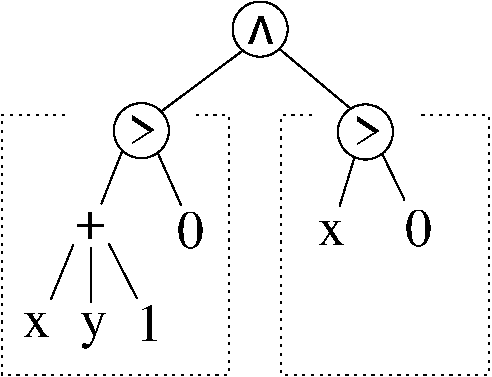
\includegraphics{relation}}\\[0.2cm]\nopagebreak
\footnotesize{\sf Fig.\ \arabic{figcount}}\\
\end{center}

In the figure above the relation $x + y +1 > 0 \wedge x > 0$ is displayed in its tree represen\-tation (e.g.\ as a parsed 
result of the string `{\tt x+y+1>0 AND x>0}'). This tree has two levels: a relation level (the encircled nodes) and an 
operation level (the nodes below the relation nodes). The relation consists of $\wedge$-Conjunction as root node with two 
{\it simple} relations ($x+y+1 > 0$ and $x > 0$, the dashed boxes in the figure) as leaves. The relation leaves contain 
the operations $x + y + 1$, $0$ and $x$, $0$. After binding $x$ and $y$ to certain numeric values, the relation can be 
evaluated, returning either {\tt true} or {\tt false}, depending on the evaluation results of the operations.\\

The approach of using tree representations for mathematical expressions is adopted by all modern Computer Algebra Systems 
(e.g.\ \cite{Wo91}, \cite{Wa91}, \cite{Mo93}), but their almost purely functional 
model allows neither typing (e.g.\ no type distinction between operations and relations)\footnote{For example, in Maple variables 
can hold relations as well as boolean or numerical values, making expressions like {\tt y = (y=1);} or 
{\tt plot(sin(true),x=0..Pi);} computable.} nor the integration in an object oriented graphical user interface.\\ 
For our requirements, we will adopt the concept of a functional representation, but merge it with an object oriented model.
This means for the architectural design that we use the different types {\tt Operation} (any symbolic expression that can 
be numerically evaluated) and {\tt Relation} (any symbolic expression that can be either true or false). We choose these 
entities because they are closed under the most transformations we will apply onto them (for example, opposed to the set
of equations -- the set of relations is closed under equivalence transformations, the set of analytic operations is closed 
under derivation), so we can still use a functional model  when transforming trees of each type.

\paragraph{Tree Representation vs. Flat Representation}
Apart from being a construct of formal languages over which human-computer interaction is possible, a tree architecture also 
grants a greater flexibility than flat structures. For example, if we want to model a finite representation of a Borel 
$\sigma$-algebra in $\mathbbm{R}$ this could be implemented by a single class, owning a list of intervals, upon which 
the operations {\tt intersect}, {\tt join}, {\tt complement} etc. are resolved. This can be quite costly if we want to 
compute the join or intersection of two Borel sets that are widely `scattered', though the user will usually test inclusion 
in the result only for some points or a single interval displayed on the screen. Also, we could not model the special case of 
infinite intervals like $\mathbbm{Z}$, $\mathbbm{R}\backslash2\pi\mathbbm{Z}$, etc. which we need when displaying periodic 
behaviours.\\
The solution to this problem is to implement the Borel set as a tree structure that has intervals and 
`periodic intervals' as leaves and operations upon Borel sets as inner nodes. When the user wants the set to be displayed
on the screen, the observed interval and an $\varepsilon$ for precision (e.g.\ pixel width) is given to the Borel set and 
a distribution of points and lines satisfying these parameters is computed.\\
As this example suggests, constructing trees of mathematical entities allows a higher degree of generalisation 
without losing flexibility and simplicity. We will also see in section \ref{model_application} that trees are easily 
transformable, adding a lot of functionality to tree-structured mathematical entities.


\subsubsection{Basic Tree Model}
All tree-organised implementations of mathematical entities share a common base class, the {\tt AbstractTreeNode}, which
offers abstract tree functionality regardless of type, like adding or removing children, searching and replacement of 
descendants, etc. From these, the basic nodes for mathematical entities are derived (at this time {\tt OpNode}, 
{\tt RelNode} and {\tt SetNode}), the subclasses of which are the concrete implementations of mathematical operations 
and operands. The tree of these nodes is referenced by the model of the mathematical entity ({\tt Operation}, {\tt Relation}, 
{\tt BorelSet}), which serves as static container and fixed reference when performing tree transformations:\\

\stepcounter{figcount}
\begin{center}
\resizebox*{14cm}{!}{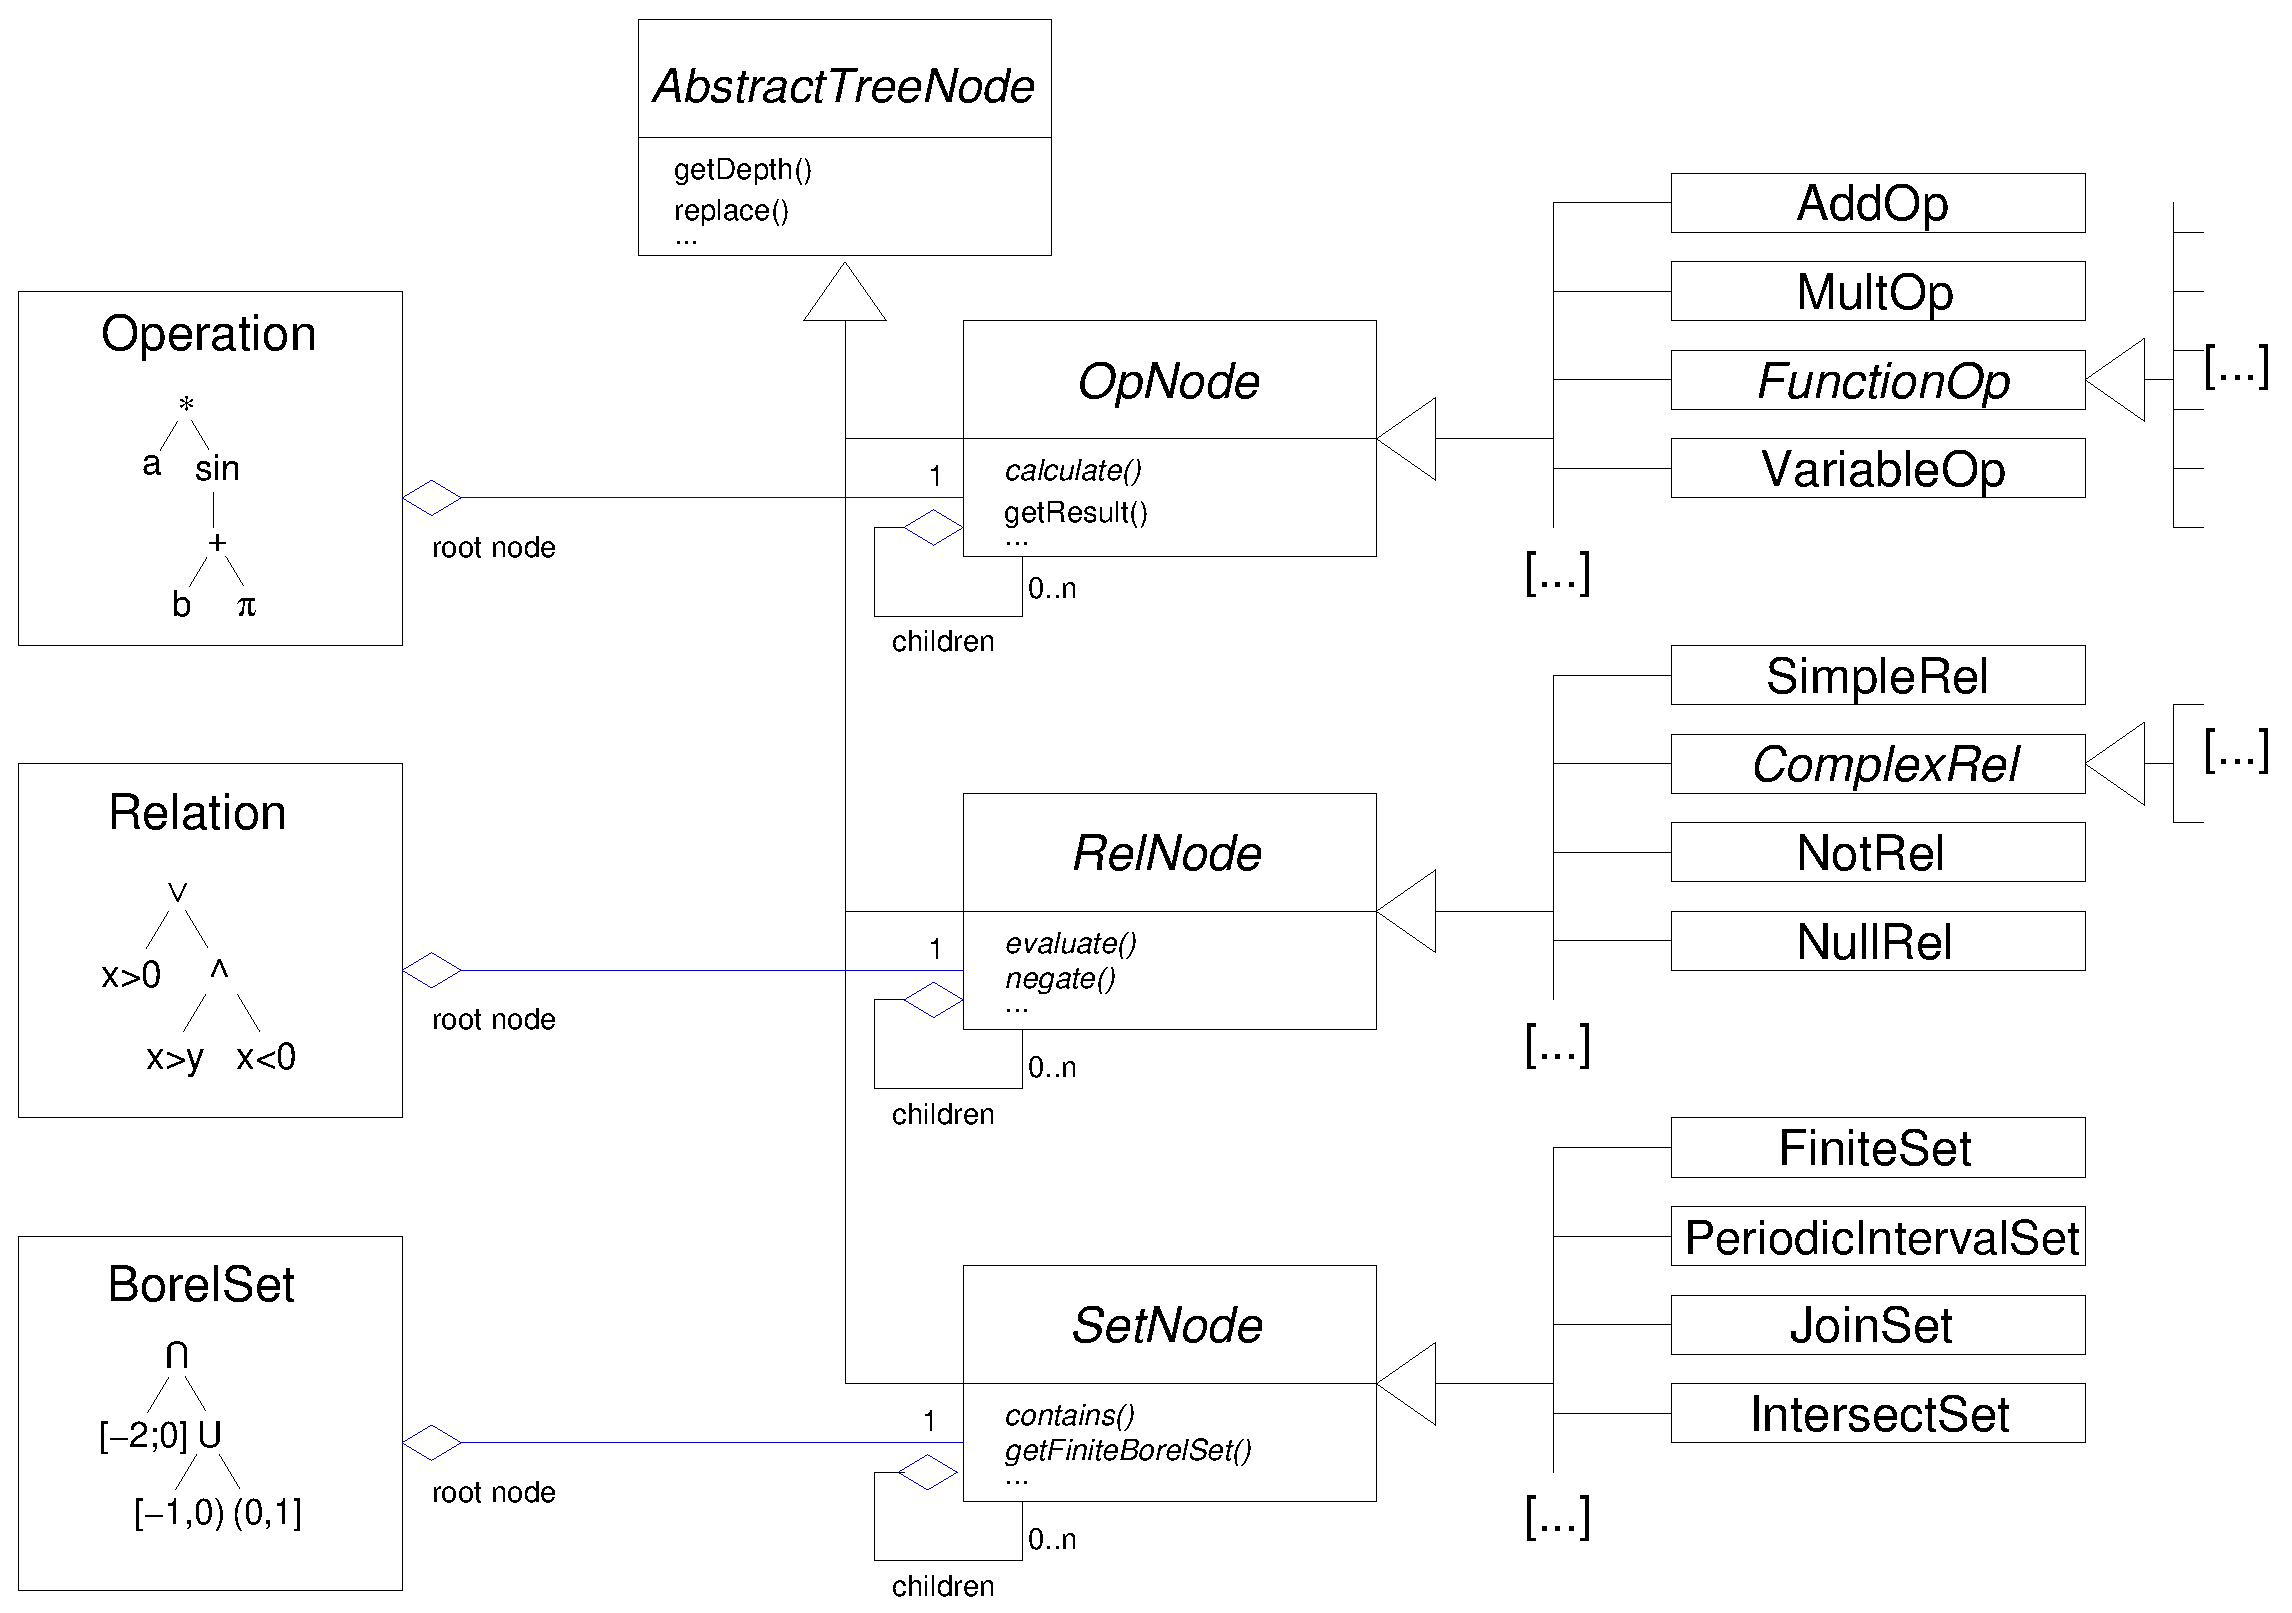
\includegraphics{treeNodes}}\nopagebreak\\[0.5cm]\nopagebreak
\footnotesize{{\sf Fig.\ \arabic{figcount}: Inheritance and aggregation model of tree nodes}}\\[0.6cm]
\end{center}

\subsubsection{Object Model of Operations}
\paragraph{Generation and Structure of Operations}
The Language {\it Op} is syntactically analysed by an recursive descent parser. When parsing an expression it creates a 
corresponding operation tree that is contained in an {\tt Operation} object. The operation tree consists of nodes that 
are of type {\tt OpNode} and whose inner nodes are functions and operations while the leaves are basically variables and 
numbers. For example, parsing the expression "sin(2x+$\pi$)" generates the operation tree {\tt (sin (+ (* 2 x) pi)}:\\

\stepcounter{figcount}
\begin{center}
\resizebox*{6cm}{!}{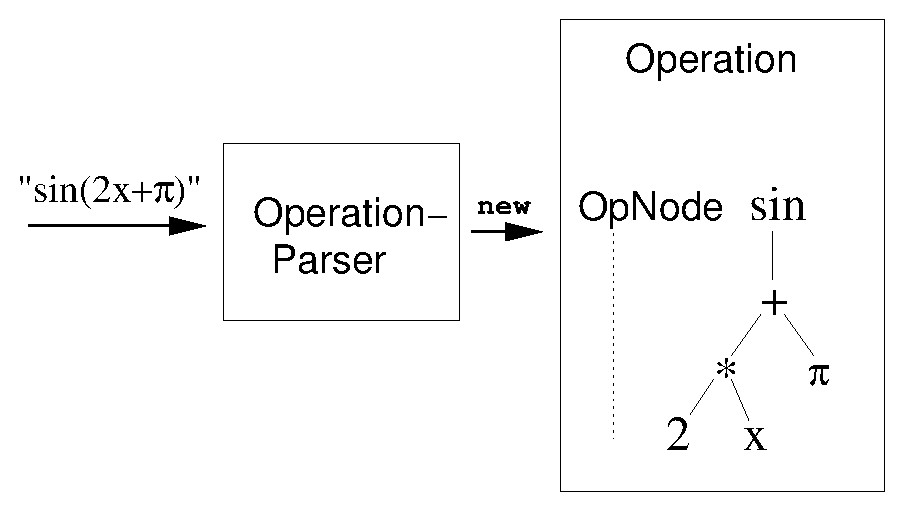
\includegraphics{op_Parser}}\\[0.2cm]\nopagebreak
\footnotesize{\sf Fig.\ \arabic{figcount}}
\end{center}

The {\tt Operation} class bundles the functionality for any operation that can be found in a function or on the left or 
right hand side of an equation, etc. It contains a reference to the operation tree and keeps track of state information 
like the variables used and normalisation status (see below).\\
The operation tree is made of instances of the class {\tt OpNode}, which is an abstract class that provides the common 
functionality for all operation nodes. It models an elementary operation with a factor and an exponent so the above 
example could also have the form {\tt (sin (+ 2x pi))}. From the functional view the factor and the exponent are not 
essentially necessary, since there are also nodes for power and multiplication operations, but with addition and 
multiplication being the most common operations, this reduces the depth of most trees. This again decreases the costs 
of analysis and synthesis of larger trees and allows a higher amount of order within the trees (for example, children 
of a multiplication node can be ordered by power, making fraction handling easier). 
Adding factor and exponent fields to an operation node is also a common technique used in CAS \cite{Bau02}.\\ 
Below, a part of the definition of {\tt algebra.op.OpNode} is shown:\\[0.3cm]

\begin{minipage}{5cm}
\end{minipage}
\begin{minipage}{12cm}
\begin{scriptsize}
\begin{verbatim}
...

public abstract class OpNode implements Cloneable, Comparable, NumberTypeDependentIF {
  ...
  /** The base value, which is calculated in {@link #calculate}. */
  protected MMNumber m_base;
  
  /**
   *  A numerical factor is stored for each operation, to reduce the tree complexity
   *  and allow group actions.
   */
  protected MMNumber m_factor;
  
  /**
   *  The exponent is stored for each operation, to reduce the tree complexity
   *  and allow group actions.
   */
  protected int m_exponent = 1;
  
  /**
   *  The children of the node, may be null (leaves), one node (e.g.\ functions) or
   *  an arbitrary number of nodes (e.g.\ multiplication).
   */
  protected OpNode[] m_children;
  
  /** The direct ancestor of this node in the Operation Tree. */
  protected OpNode m_parent;
  
  /** The number class being used. */
  protected Class m_numberClass;

  ...
\end{verbatim} 
\end{scriptsize}
\end{minipage}


\paragraph{Operation Transformations and Normal Form}
\label{transformations}
As mathematics often consists of transforming expressions, operations can be transformed in multiple ways.
For example, the addition of the number 3 to an existing operation can be done by creating a new addition 
node that has the old operation tree and a '3'-node as children and taking the addition node as the root node 
for the new operation. There are of course many other possible transformations like substitution, separation 
of variables, factorisation, derivation, etc. To implement these in an object model, a two level approach is 
used: Transformations that create a new operation tree with specific rules for each node (like calculating 
the derivative or the inverse) are handled by the node object itself, whereas transformations that alter the 
existing tree structure (expansion, simplification, etc.) are handled by a transformer facility called 
{\tt OpTransform}. This two-level approach allows to combine the power of recursive algorithms with the 
structural advantage of object-orientation.

\stepcounter{figcount}
\begin{center}
\resizebox*{12cm}{!}{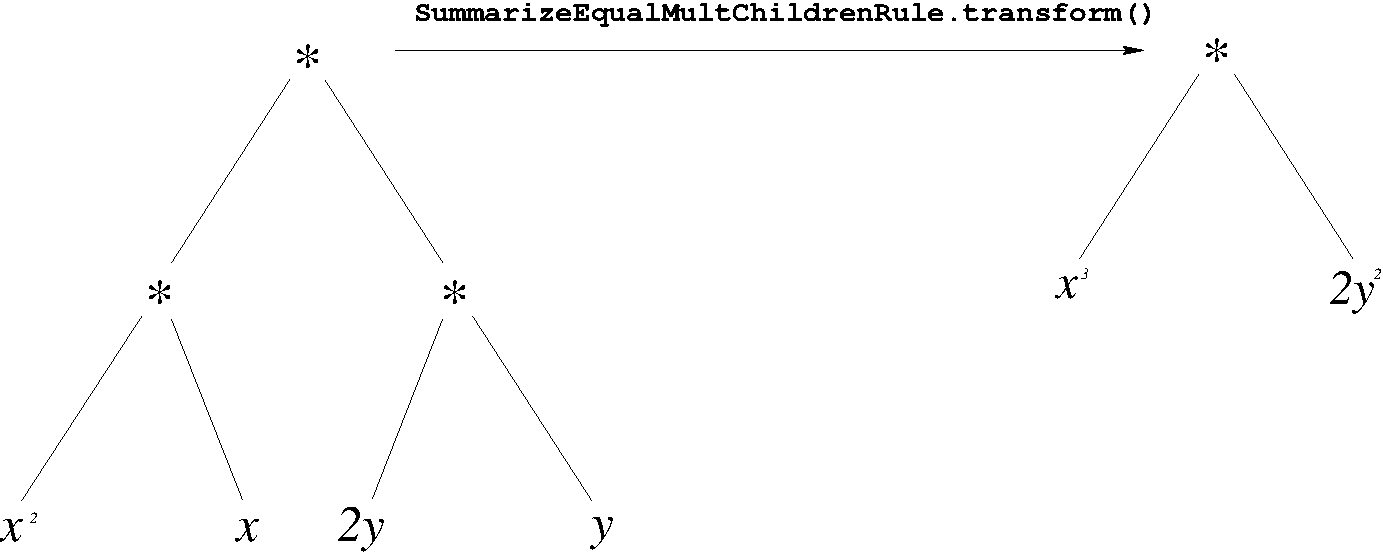
\includegraphics{expressionTransform}}\nopagebreak\\[0.5cm]\nopagebreak
\scriptsize{{\sf Fig.\ \arabic{figcount}: Transformation of a subtree by a rule}}\\[0.6cm]
\end{center}

The {\tt OpTransform} object is a tree automaton that transforms trees by using a set of rules (located in the subpackage 
{\tt algebra.op.rule}), which specify a certain subtree pattern and a transformation that 
is performed if the tree matches the pattern.\\

For example, in the tree {\tt (* (* x$^2$ x) (* 2y y))} (see figure) the condition for a multiplication node containing two 
or more equal children (without regarding their factors or exponents) applies to both '{\tt *}' children of the root node. 
The rule object therefore raises the power of the first child by the number of the other children, transforming the tree 
to {\tt (* x$^3$ 2y$^2$)}. This would also apply to the root node if a previous application of {\tt CollapseEqualOpsRule} 
had flattened the tree to {\tt (* x$^2$ x 2y y)}.

In order to apply a rule like in the example above, a certain structure of the tree has to be assumed. For example, 
the tree {\tt (* (* (\^{} x 2)) x)} is mathematically equivalent to {\tt (* x$^2$ x)}, but it is harder to analyse and
transform. Because the rules should be kept as simple as possible (since there are many of them and their set should be 
easily expandable), it is reasonable to specify a normal form for operation trees.\\
The normalisation rules are located in {\tt algebra.op.rule.normalize}. Here are some examples:\\[0.3cm]

\begin{small}
\begin{tabular}{ll} 
Name & Application Example\\
{\tt NormalizeMultRule} & {\tt (* 4x 6y) $\rightarrow$ 24(* x y)}\\
{\tt NormalizeExponentsRule} & {\tt (* x$^4$ y$^6$) $\rightarrow$ (* x$^2$ y$^3$)$^2$}\\
{\tt CollapsePowerRule} &  {\tt  (\^{} (\^{} x y) z) $\rightarrow$ (\^{} x (* y z))}\\
{\tt HandleFunctionSymmetryRule} & {\tt (sin -x) $\rightarrow$ -(sin x)}\\
\end{tabular}\\[0.3cm]
\end{small}

This set can be easily expanded, most of the rules consist of less than 20 lines of code.
All the rules are applied in a deterministic order and since they always produce defined results, it can be ensured 
that after none of the rules can be applied to any node in the tree anymore, the operation has a unique defined form.
This form is defined as the normal form of the operation (for the specific rule-set). Trees having the same normal form 
are considered to be mathematically equal by the system.

\subsubsection{Object Model of Relations}
\paragraph{Generation and Structure of Relations}
Analogous to operations, relations are usually generated by parsing a word of {\it Rel} (see the grammar in 
\ref{rel_grammar}) and by constructing a relation tree composed of {\tt RelNode}s. The inner nodes of the relation tree 
are the logical operations 
$\vee$, $\wedge$ and $\neg$, while the leaves are either
simple relations (equations or inequations) or special nodes like {\tt AllRel} and {\tt NullRel}, which either relate 
everything (making interpretation of the used domain necessary) or nothing.

\paragraph{Transformation of Relations, Normal Form}
Like operations, relations can be transformed in multiple ways, the most used transformations are the logic
transformations that negate, conjunct or disjunct subtrees. But there are also complex transformations that occur when a
simple relation is transformed. For example, if the inequation $x^2 - x > 0$ is divided by $x$ this leads to the
equivalent complex relation\\ $x-1 > 0 \wedge \frac{1}{x} > 0 \vee x-1<0 \wedge \frac{1}{x} < 0$ (see figure).\\[0.3cm]
The functionality for handling relation transformations and its special cases are implemented in the class 
{\tt RelTransform}.\\

\stepcounter{figcount}
\begin{center}
\resizebox*{12cm}{!}{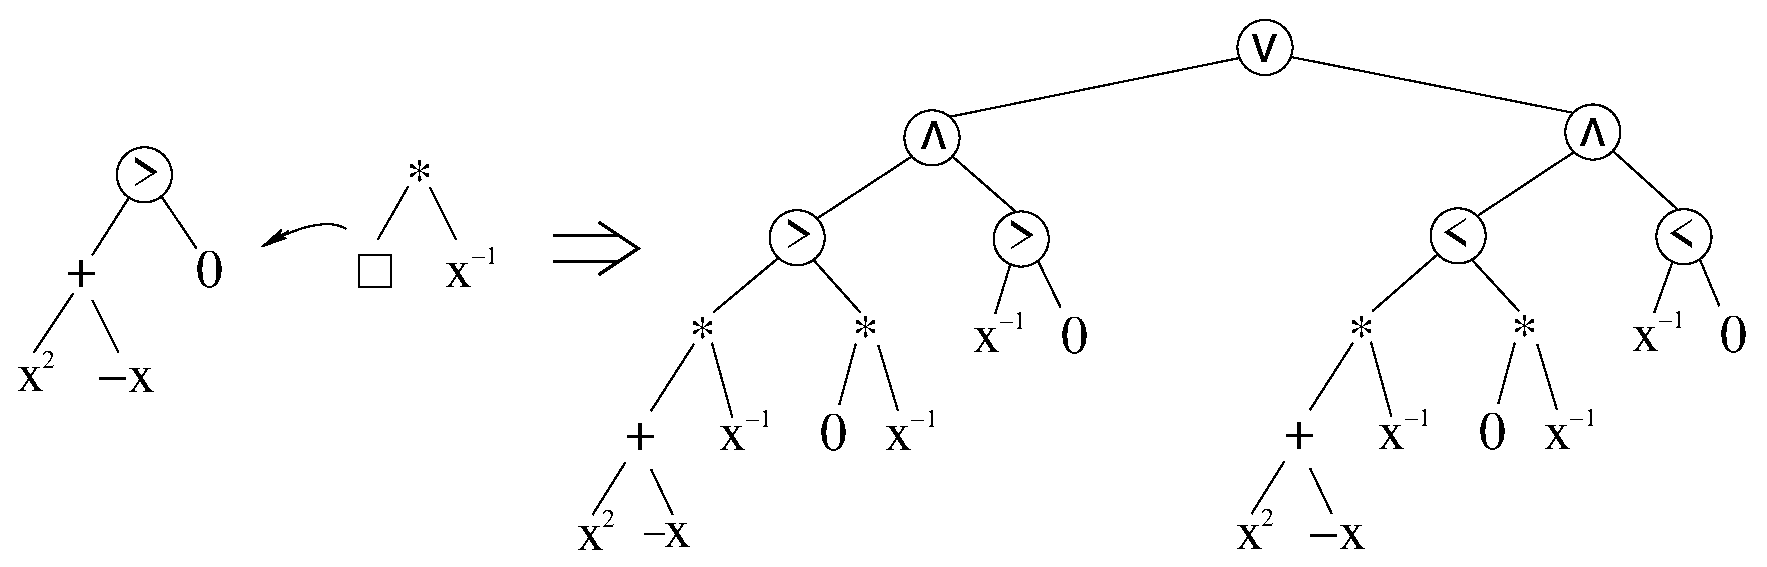
\includegraphics{relationTransform}}\nopagebreak\\[0.5cm]\nopagebreak
\footnotesize{{\sf Fig.\ \arabic{figcount}: Transformation of a relation}}\\[0.6cm]
\end{center}

For comparation and simplification of relations, again, a higher order is needed for the trees to facilitate 
the development of tree analysis and transformation code.\\
For example, the relation $x = y \wedge y = x$ should be recognised as redundant by the system and be 
simplified to $x = y$. As for operation trees, this is done by defining a normal form for relations and
implementing rules for normalisation.\\ 
The normalisation rules are located in {\tt algebra.rel.rule.normalize}.
Here are some examples:\\[0.3cm]
\begin{small}
\begin{tabular}{ll} 
Name & Application Example\\
{\tt MoveOrUpwardsRule} &  {\tt [[x=0 OR y=0] AND z=0] $\rightarrow$ [x=0 AND z=0] OR [y=0 AND z=0]}\\
{\tt CollapseComplexRule} & {\tt [[x=0 AND y=0] AND [z=0] $\rightarrow$ [x=0 AND y=0 AND z=0]}\\
{\tt RemoveNotRelRule} & {\tt [NOT [x>=y]] $\rightarrow$ [x < y]}\\
\end{tabular}\\[0.3cm]
\end{small}


\subsection{Applications}\label{model_application}
To demonstrate the practical use of the algebraic object model, we give two application examples.

\paragraph{Symbolic Derivation}
The symbolic derivative of a differentiable function can be computed automatically by simply applying 
the well known rules for elementary functions and chaining them together for compound functions, using the
derivation rules for sums, products and compositions.\\


\stepcounter{figcount}
\begin{center}
\resizebox*{12cm}{!}{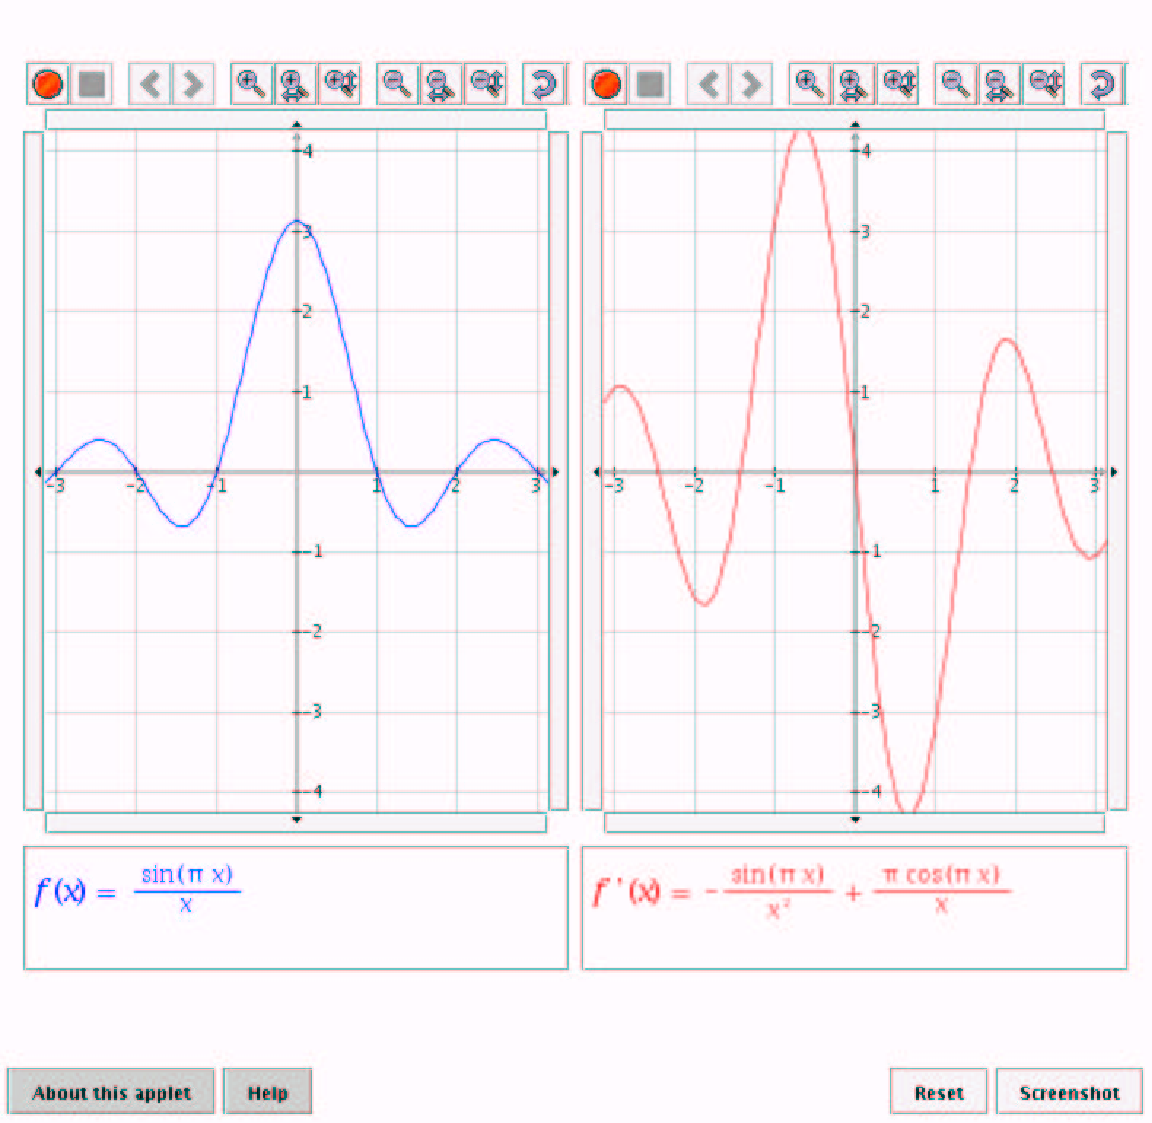
\includegraphics{functionAndDerivative}}\nopagebreak\\[0.5cm]\nopagebreak
\footnotesize{{\sf Fig.\ \arabic{figcount}: The function and derivative plotter}}\\[0.6cm]
\end{center}

The application presented to the user is an applet that plots an arbitrary function typed in by the user and additionally
computes and displays the derivative (if any exists).\\[0.3cm]

\stepcounter{figcount}
\begin{center}
\resizebox*{6cm}{!}{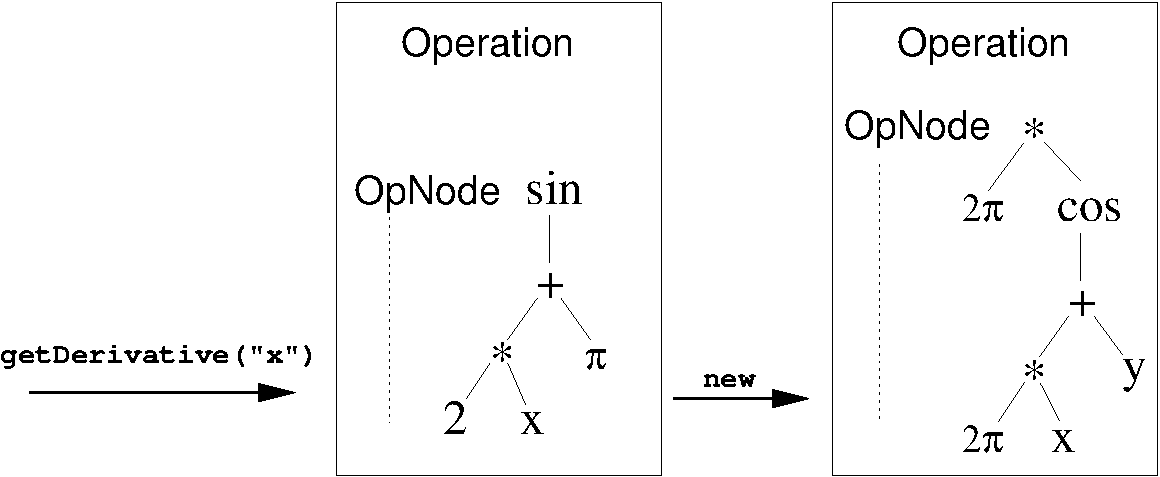
\includegraphics{op_derive}}\nopagebreak\\[0.5cm]
\nopagebreak
\footnotesize{{\sf Fig.\ \arabic{figcount}: Object model for deriving operations}}\\[0.6cm]
\end{center}

From a technical perspective this is done by using an {\tt MMFunctionDefinedByOperation} object from which another instance 
is created with an {\tt Operation} that is returned by the {\tt getDerivative()} method of the first operation.\\
Deriving an operation can be implemented completely on a per-node basis, therefore the method {\tt Operation.getDerivative()} 
simply delegates the calculation to the root node of the operation tree. The derivation code of an operation node 
has two parts: a generic part that does the derivation for the internal factor and exponent and a specific part that 
varies on the node type. Below is a code snippet containing the node specific derivation code in the class 
{\tt SinOp}:\\[0.3cm]


\begin{minipage}{5cm}
\end{minipage}
\begin{minipage}{12cm}
\begin{scriptsize}
\begin{verbatim}
  /**
   *  Implements <i> (sin(f(x)))' = cos(f(x)) * f`(x) </i>.
   */
  public OpNode getDerivative(String variable){
    
    if(getMaxPowerOfVariable(variable) == 0)
      return new NumberOp(m_numberClass, 0);
    
    // cos(f(x))
    OpNode cosOp = new CosOp(m_numberClass);
    cosOp.setChildren(new OpNode[]{(OpNode)(m_children[0].clone())});
    
    // f'(x)
    OpNode derivedChild = m_children[0].getDerivative(variable);
    
    // cos(f(x)) * f'(x)
    MultOp derivedCosOp = new MultOp(m_numberClass);
    derivedCosOp.setChildren(new OpNode[]{cosOp, derivedChild});
    return deriveNode(derivedCosOp);
  }
\end{verbatim} 
\end{scriptsize}
\end{minipage}\\[0.3cm]

The generic part implemented in the abstract class {\tt OpNode} is as follows\\

\begin{minipage}{5cm}
\end{minipage}
\begin{minipage}{12cm}
\begin{scriptsize}
\begin{verbatim}
  /**
   *  Implements <i>(m*a(x)^n)' = (n*a(x) ^ (n-1) * m*a'(x)</i>.
   *  @param derivedNode a'(x)
   */
  protected OpNode deriveNode(OpNode derivedNode){
    if(m_exponent == 1){
      derivedNode.setFactor(m_factor.copy());
      return derivedNode;
    }
    MultOp derivedPower = new MultOp(m_numberClass);
    OpNode newPower = (OpNode)clone();
    newPower.m_factor.mult(NumberFactory.newInstance(m_numberClass, m_exponent));
    newPower.m_exponent--;
    derivedPower.setChildren(new OpNode[]{newPower, derivedNode});
    return derivedPower;
  }
\end{verbatim} 
\end{scriptsize}
\end{minipage}\\[0.3cm]


\paragraph{Definition Range of Operations}
\label{definition_range_operations}
Another useful application of the MathletFactory algebraic object model is the ability to compute the definition 
range of an operation. We have used this functionality to add an extra warning when displaying mathematical entities
that use operations which are only partially defined.\\
When determining definition gaps, it poses a serious implementation problem to numerically calculate the complete 
definition range and display it graphically for any function (as the example $f(x) =  \frac{1}{\sin(\frac{1}{x})}$ in the
figure below shows).\\
The MathletFactory addresses this problem by displaying the definition range of a function as a symbolic expression. 
Though this expression often has an implicit form (showing only a relation of the used variables that must be satisfied) 
the user is warned of existing definition gaps, and he is principally able to find out where they are.\footnote{Also, by 
using the {\tt Relation.toContentMathML()} export method, an application programmer is able to link it with a computer algebra 
system or to implement a numerical solution of his own.}\\[0.3cm]

\stepcounter{figcount}
\begin{center}
\resizebox*{8cm}{!}{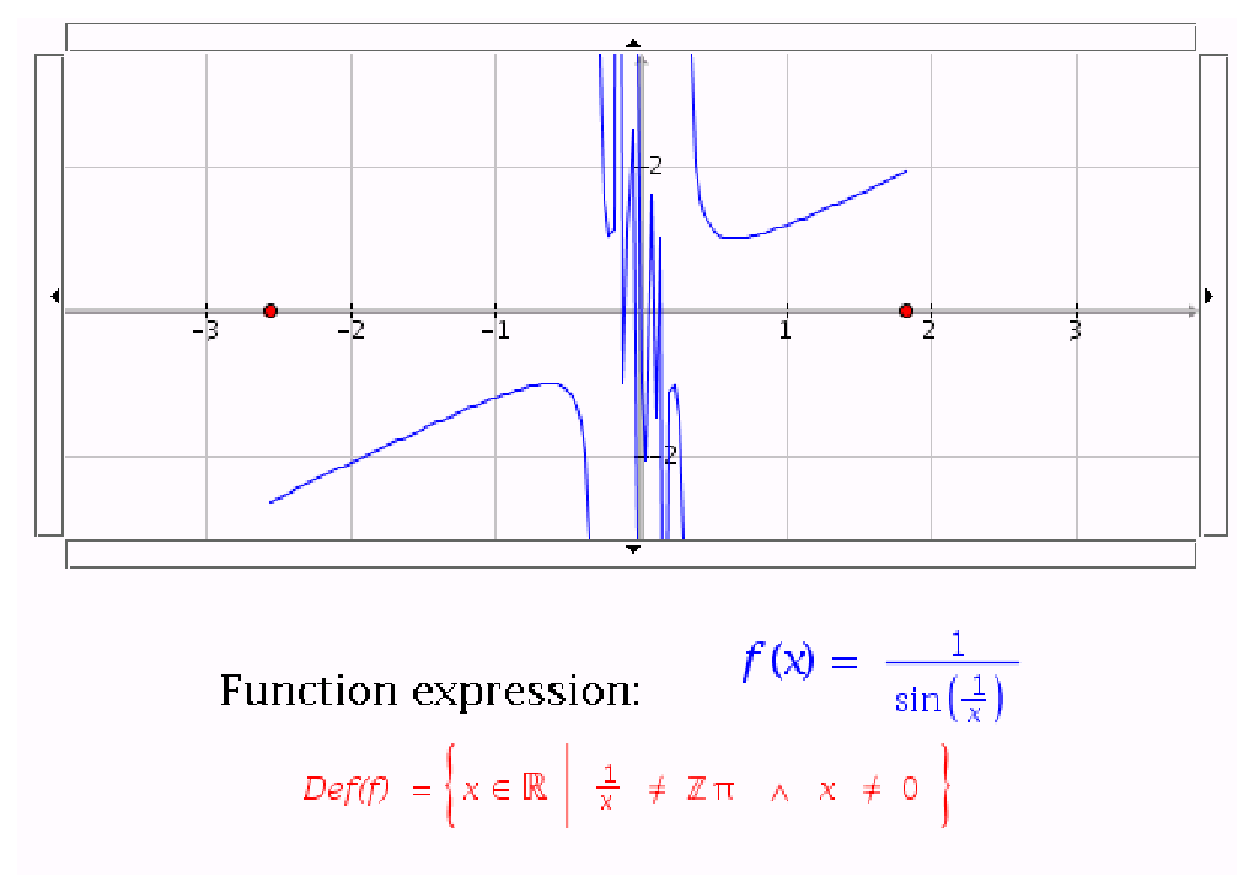
\includegraphics{simplefunctionplotter2}}\nopagebreak\\[0.5cm]\nopagebreak
\footnotesize{{\sf Fig.\ \arabic{figcount}: The function plotter with definition range detector}}\\[0.6cm]
\end{center}

From the technical perspective the computation of the definition range for an arbitrary operation is also solved on a
per-node basis. By calling the method {\tt getDefinedRel()} the {\tt OpNode} object creates a {\tt RelNode} object which
represents a relation that a member of the definition range for the operation must satisfy. 
The {\tt RelNode}s of the children of an {\tt OpNode} are connected by an {\tt AndRel} conjunction, forming a relation tree
that is at last anchored in a {\tt Relation} object by the enclosing {\tt Operation.getDefinedRelation()} method.
For the {\tt OpNode}s there is -- like the computation of the derivative -- a generic and a node-specific implementation.
The generic part, implemented in {\tt OpNode} is as follows:\\[0.3cm]

\begin{minipage}{5cm}
\end{minipage}
\begin{minipage}{12cm}
\begin{scriptsize}
\begin{verbatim}
  /**
   * Returns the relation for which the operation represented by this node is defined.
   * @see #getDefinedRel(OpNode operand)
   */
  public RelNode getDefinedRel(){
    
    // by default the operation is defined totally for any variable
    RelNode definedRel = new AllRel(m_numberClass);
    
    // retrieve the definition range of this node with the child as argument
    // (non unary operations overload this method)
    if(m_children != null)
      definedRel = getNodeDefinedRel(m_children[0]);
      
    // for nodes with a negative exponent the base may not become zero
    if(getExponent() < 0){
      OpNode nodeWithoutExponent = (OpNode)clone();
      nodeWithoutExponent.setExponent(1);
      definedRel = new AndRel(definedRel, new NotRel(nodeWithoutExponent.getZeroRel()));
    }    
    
    // intersect the defintion range of this node with the definion range of the children 
    if(m_children == null)
      return definedRel;
    else
      return new AndRel(definedRel, getChildrenDefinedRel()); 
  }

  /**
   * Returns the relation subtree for which this operation with 
   * <code>operand</code> as child is defined. It does not consider the 
   * exponent of this node, which is be checked in {@link #getDefinedRel}.
   */
  public abstract RelNode getNodeDefinedRel(OpNode operand);
\end{verbatim} 
\end{scriptsize}
\end{minipage}\\[0.3cm]
The specific part is implemented by the subclasses of {\tt OpNode} in {\tt getNodeDefinedRel()}. Here is an example for 
{\tt TanOp} returning a relation that says that the cosine of its operand may not be zero:\\[0.3cm]
\begin{minipage}{5cm}
\end{minipage}
\begin{minipage}{12cm}
\begin{scriptsize}
\begin{verbatim}

  public RelNode getNodeDefinedRel(OpNode operand){
    return new NotRel(new CosOp(m_numberClass).getZeroRel((OpNode)operand.clone()));
  }

\end{verbatim} 
\end{scriptsize}
\end{minipage}\\[0.3cm]

\subsection{Arithmetic and Geometric Symbolic View Architecture}
One pattern that has been consequently used in the development of the symbolic view architecture is, that every
mathematical inclusion is transformed to a `containedness' relation on the view component level. This allows an
easy development and support for a multitude of symbolic representations. We illustrate this with the example
of constructing the parametric view for an affine plane in $\mathbbm{R}^3$:

\stepcounter{figcount}
\begin{center}
\resizebox*{6cm}{!}{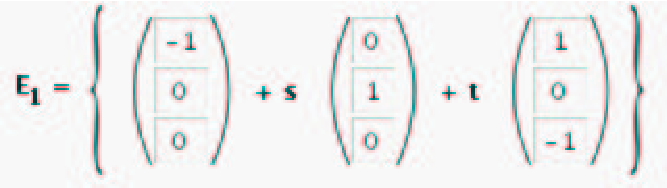
\includegraphics{plane_symbolic}}\hspace{1cm}\resizebox*{5.5cm}{!}{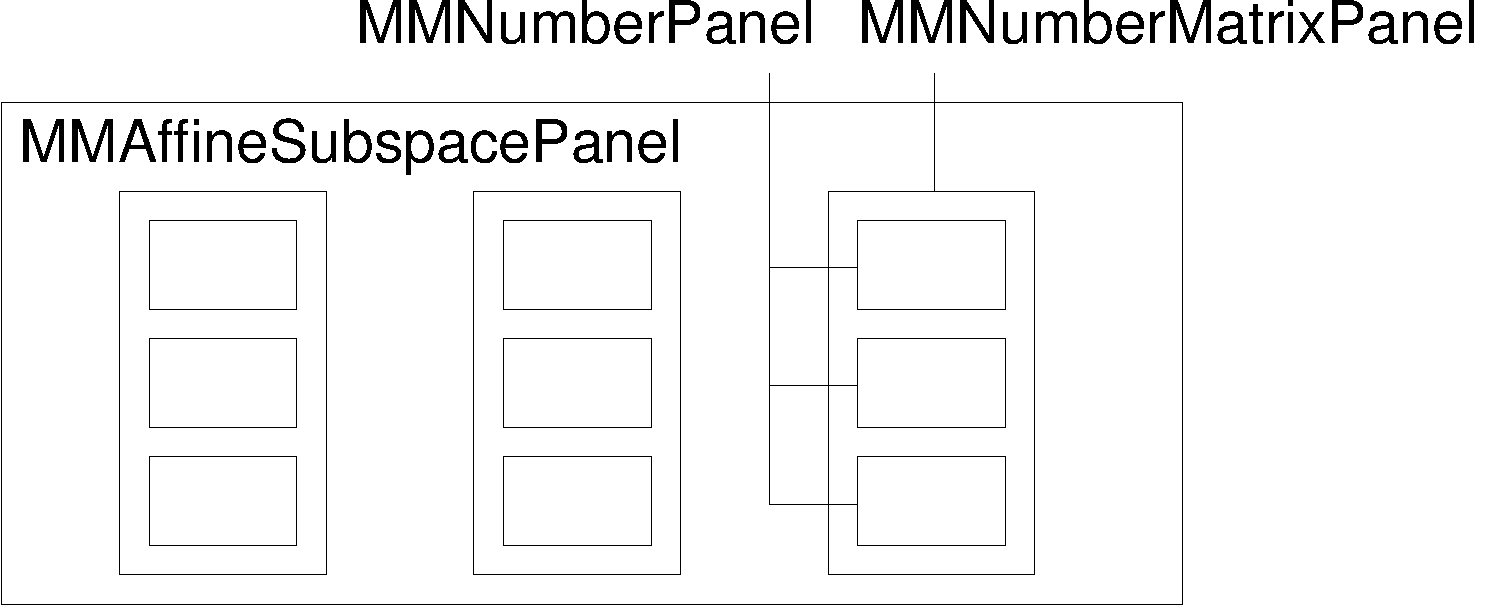
\includegraphics{plane_symbolic_structure}}\nopagebreak\\[0.3cm]\nopagebreak
\footnotesize{{\sf Fig.\ \arabic{figcount}: The symbolic view of a plane and its structure}}\\[0.6cm]
\end{center}

On Java level, the view is simply a subclass of {\tt JPanel}, namely an {\tt MMAffineSubspacePanel}. This class
acts not only as a view for a plane in $\mathbbm{R}^3$, but also for a line or point in $\mathbbm{R}^3$ or in 
$\mathbbm{R}^2$, thus making it possible to use it as a view of a dynamically generated affine subspace (like the
intersection or join of other affine spaces). But let us first consider, that it displays a regular (non-degenerated)
plane. In this case, we need to display three vector displays: one displaying the origin vector and two for the 
direction vectors. This is simply done by adding three {\tt MMNumberMatrixPanel}s, which is the standard display
component for a vector of any dimension, but also of course for any number matrix of arbitrary form. These panels
in turn contain all entries as {\tt MMNumberPanel}, the symbolic representation for numbers of any 
type.\footnote{Note, that the inclusion does not end there, for the number panel itself contains an operation panel 
(see below) to allow the display of constants like $\frac{3}{2}pi$, etc.} A simple update mechanism using the Java 
property support ensures, that changes performed by the user are recorded by the master MMObject. On the other hand, 
if the mathematical state of the MMObject changes (e.g.\ by updating or user interactions on the graphical level), 
the changes are immediately displayed, allowing the user to continuously watch the symbolic perspective of his 
actions.\\
This applies not only to changing the vectors of the affine subspace, but also to changing its dimension: If the
plane was the result of an intersection of two other planes (which were geometrically identical) and one of these 
planes changed, making the intersection a line or an empty space, the symbolic view adapts to these cases without
complaints.

\subsection{Algebraic Symbolic View Architecture}
In the following, we will also sketch the view architecture used by the MathletFactory's algebraic object model, 
for details the commented source code and API documentation should be consulted.\\
The architecture for symbolically displaying algebraic entities is closely related to the structure of the algebraic 
object model: A tree of operation nodes is mapped on a tree of view nodes that recursively draw the expression on a 
panel, whereas a tree of relation nodes is mapped on a tree of panels with each parent containing its children.

\subsubsection{View Architecture of Operations}
\label{view_model}
The implementation of the symbolic view for an operation is the {\tt OperationPanel}. This is a GUI component that 
draws the expression string on its screen area when asked to repaint. This is done by view nodes (an analogon to the 
\TeX{} noads\footnote{\cite{Kn82}}), each of which corresponds to an operation node of the {\tt Operation}. Apart from 
the reference to its operation node, a view node keeps track of its metrics which is determined by the metrics of its 
children (if any) and the font of the panel. For example, the view node for a square root must know the width and height 
of its child expression in order to fully enclose the radicand (see figure).\\
So when a repaint event is sent to the operation panel, the panel asks its root view node to draw itself on the panel.
If the root view node has children, it asks them to calculate their metrics (which in turn may depend on their children�s
metrics, etc.) and then draws the expression it represents accordingly.\\

\stepcounter{figcount}
\begin{center}
\resizebox*{6cm}{!}{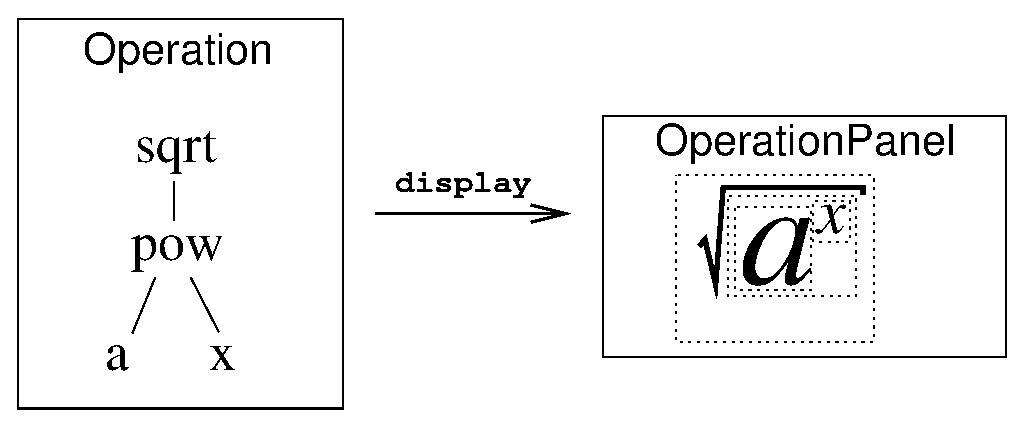
\includegraphics{opView}}\nopagebreak\\[0.5cm]\nopagebreak
\footnotesize{{\sf Fig.\ \arabic{figcount}: Displaying operations, the dashed lines mark the {\tt OpViewNode}s that draw on the {\tt OperationPanel}.}}\\[0.6cm]
\end{center}

\subsubsection{View Architecture of Relations}
The inclusion of operations in relations can also be transferred to the view architecture: The view component for a simple
relation, a {\tt SimpleRelationPanel} is merely a panel containing two {\tt OperationPanel}s with a relation sign label 
between them. Complex relations are displayed by instances of {\tt RelationContainer}: Panels that contain either 
{\tt SimpleRelationPanel}s or other {\tt RelationContainer}s. The root node itself is contained in a component called
{\tt RelationPanel}.\\

\stepcounter{figcount}
\begin{center}
\resizebox*{6cm}{!}{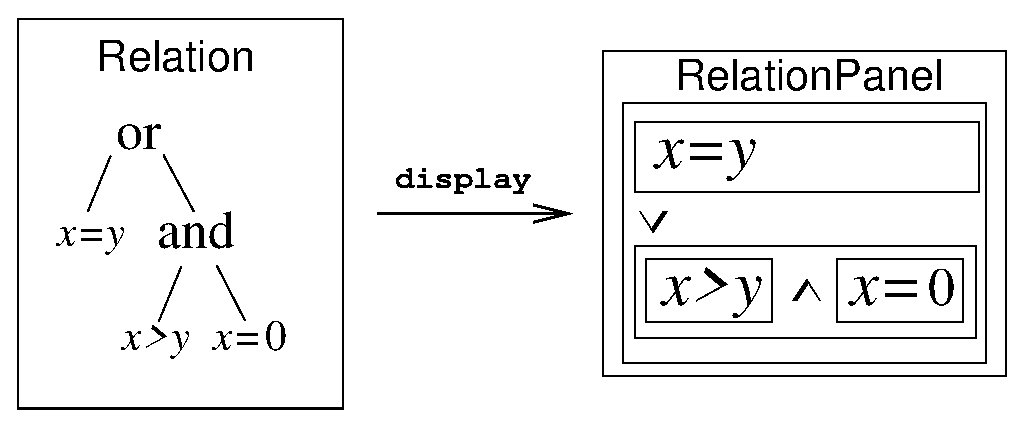
\includegraphics{relView}}\nopagebreak\\[0.5cm]\nopagebreak
\footnotesize{{\sf Fig.\ \arabic{figcount}: Relation trees are rendered in a container hierarchy rooted by an {\tt RelationPanel}.}}\\[0.6cm]
\end{center}

\subsubsection{Metrics of View Components}
The MathletFactory uses the standard metrics model of typography\footnote{\cite{He93}}: The metrics of each glyph is 
characterised by its width, ascent and descent; for the rendering of fractions, sub- and superscripts the baseline must 
also be recorded. Operation view nodes keep their metrics parameters in an object called {\tt ViewNodeMetrics}. 
On the panel level (anything that uses {\tt OperationPanel}s or container trees of these) this is done by implementing 
the interface {\tt Alignable}, which declares methods for retrieving the metrics parameters. By using this interface it is 
ensured that two operations can be horizontally aligned (i.e.\ having the same baseline), even if they have different 
heights or one of them has a border (e.g.\ for marking it as editable).\\

\stepcounter{figcount}
\begin{center}
\resizebox*{8cm}{!}{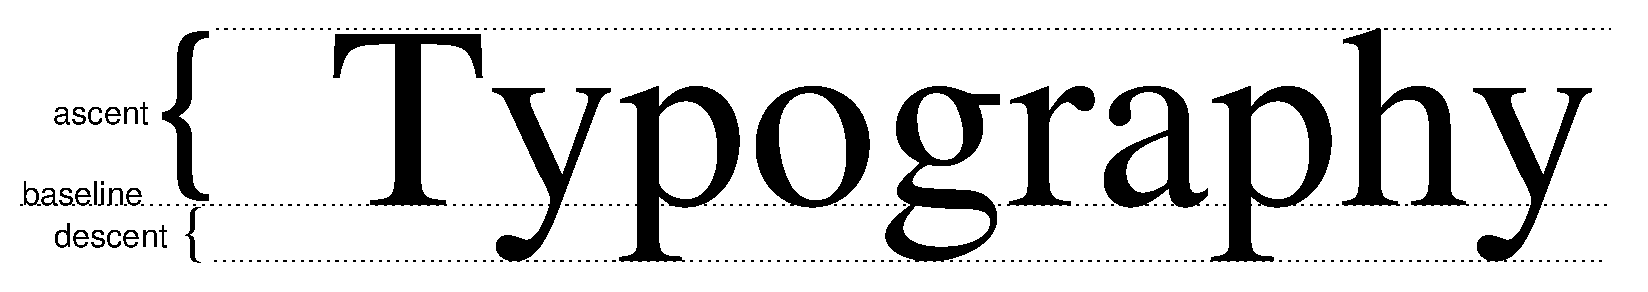
\includegraphics{typo}}\nopagebreak\\[0.5cm]\nopagebreak
\footnotesize{{\sf Fig.\ \arabic{figcount}: The baseline, ascent and descent of a font.}}\\[0.6cm]
\end{center}

\subsection{Graphical View and Controller Architecture}

At the time of writing, implementations for the Java2D system library and the Java3D API exist, but previous prototype 
implementations have also been tested with the third party graphics library JavaView\footnote{\cite{JV04}}. The 
architecture works as follows: For each different display type there exists a specific canvas (a subclass of 
{\tt MMCanvas}) that can be added to an applet like any other GUI component. If an application programmer wants to display 
a certain MMObject, he simply calls {\tt addObject(MMObjectIF object)} in the canvas with the MMObject as argument and the 
systems automatically assigns the appropriate (or a previously chosen) visual representation.\\

\stepcounter{figcount}
\begin{center}
\resizebox*{7.5cm}{!}{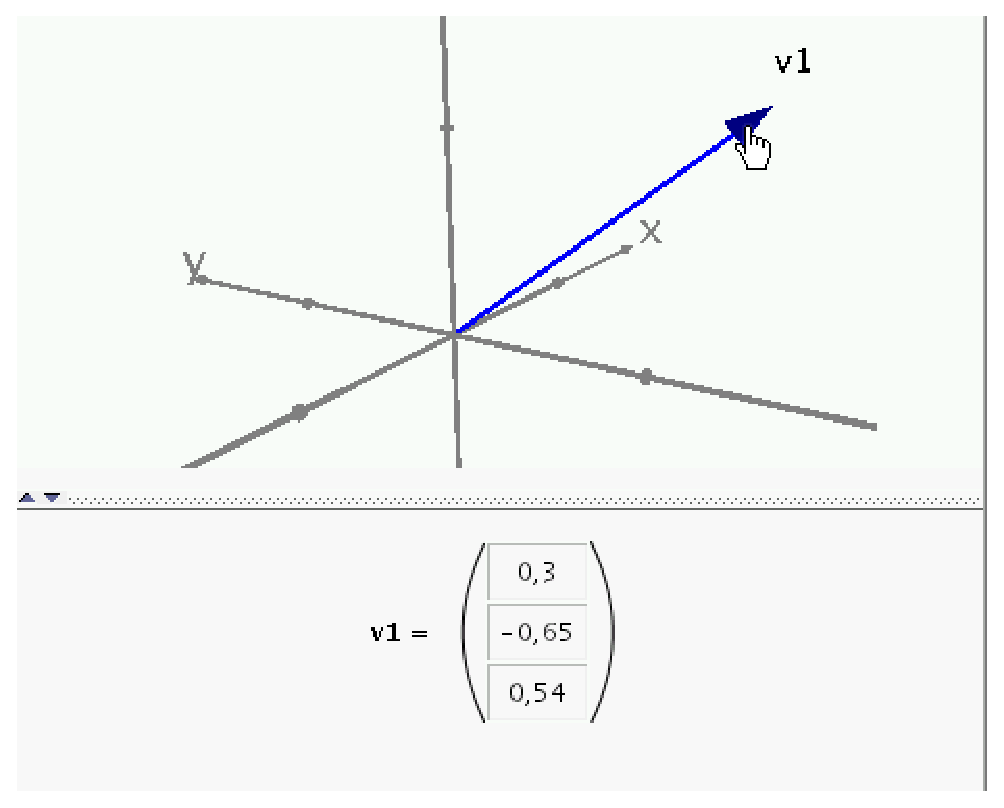
\includegraphics{3d_vector}} \hspace{1.5cm}
\resizebox*{7.5cm}{!}{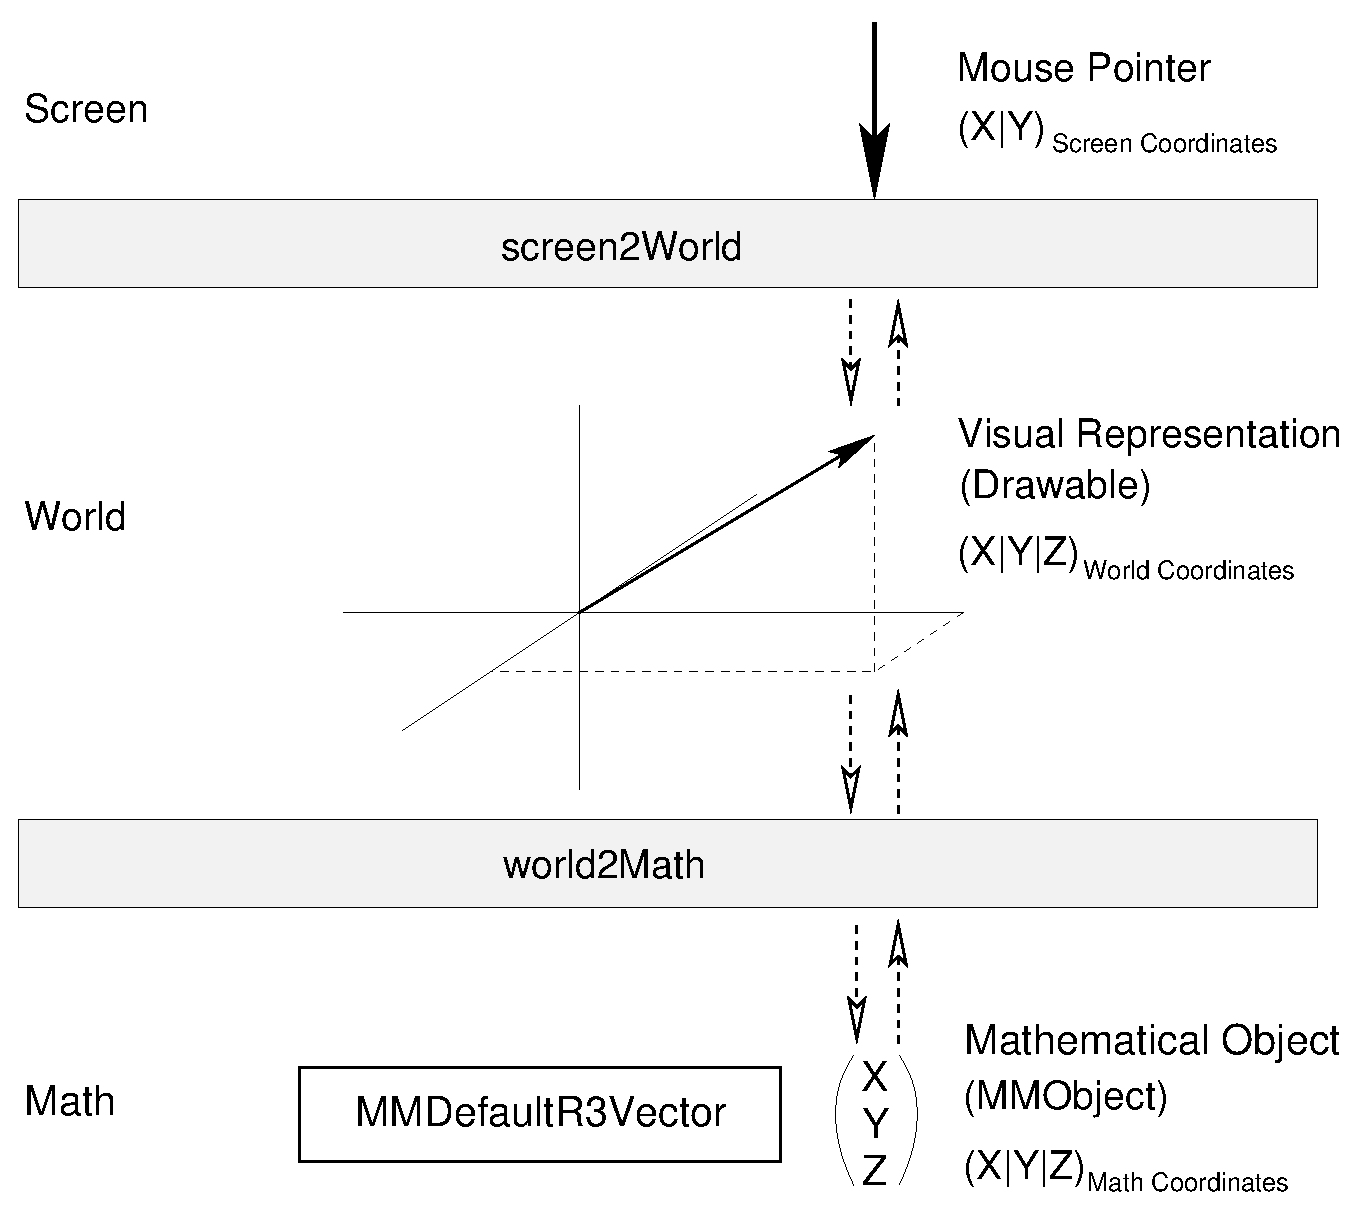
\includegraphics{vector_drag}}\nopagebreak\\[0.5cm]\nopagebreak
\footnotesize{\sf Fig.\ \arabic{figcount}: Dragging a 3D vector: How the display and interaction system works}\\[0.6cm]
\end{center}

For example, when a user drags the end point of a 3D vector with the mouse, the mouse coordinates (measured in pixels) 
are transformed by a matrix {\tt screen2World} into world coordinates. These describe a virtual space, where the visual 
representations of mathematical objects `live'. The mathematical objects themselves reside in a separate coordinate space 
called the math space. This allows them to be independent of the worlds geometry and dimension, thus allowing, for example, 
projections from a spherical geometry into the euclidian world coordinate space. For euclidian math spaces the 
transformation is simply done by another matrix called {\tt world2Math}. So when the user drags the vector, the mouse 
coordinates are transformed into world and math coordinates. The object's coordinates are changed and the graphical view 
updates accordingly, allowing further interaction. For 2D (or 1D) vectors the mechanism is the same.\\

We have given only a short overview of a complex system; yet, an application developer needs not know about all this, 
because there is a large set of prefabricated {\it handlers} that implement almost all desired functionality for 
manipulating MMObjects. So if an application developer wants to construct a mathlet, where the user may drag a vector (or 
any other MMObject), he only has to add the appropriate handler to it.

\begin{thebibliography}{100}  

\bibitem[ASU86]{ASU86} A: Aho, R. Sethi, J. Ullman. Compilers - Principles, Techniques and Tools. Addison Wesley. 1996.

\bibitem[Bau02]{Bau02} C. Bauer, A. Frink, R. Kreckel.\\
Introduction to the GiNaC Framework for Symbolic Computation within the C++ Programming Language.\\
Journal of Symbolic Computation Volume 33, Number 1, 2002.

\bibitem[Bu96]{Bu96} F. Buschmann et al. Pattern-Oriented Software Architecture, Volume 1: A System of 
Patterns. Addison-Wesley 1996.

\bibitem[Co03]{Co03} H. Comon et al. Tree Automata Techniques and 
Applications. Preprint, 2003.\\ {\footnotesize {\sf http://www.grappa.univ-lille3.fr/tata}}

\bibitem[He93]{He93}  R. Hersch (Ed.). Visual and Technical Aspects of Type. Cambridge University Press. 1993.

\bibitem[HU79]{HU79}J.E. Hopcroft and J.D. Ullman. Introduction to Automata
Theory, Languages and Computation. Addison Wesley. 1979.

\bibitem[JV04]{JV04} JavaView homepage. 2004.\\
{\footnotesize {\sf http://www.javaview.de}}

\bibitem[Kn82]{Kn82} D. Knuth. Documented \TeX{} source code. 1982.\\
{\footnotesize {\sf http://www.ctan.org/tex-archive/systems/knuth/tex/tex.web}}. 

\bibitem[Mo93]{Mo93} K. Morisse. Datenstrukturen und Speicherverwaltung in MuPAD. In: 
mathPAD Vol. 3 No. 2. 1993.\\
{\footnotesize {\sf http://www.mupad.de/mathpad.shtml}}

\bibitem[Wa91]{Wa91} Maple Language Reference Manual. Waterloo Maple Publishing. 1991.

\bibitem[Wo91]{Wo91} S. Wolfram. The Mathematica Book. Cambridge. 1991.

\end{thebibliography}

\end{document}
